\documentclass{cmspaper}
\usepackage{booktabs}
\usepackage{graphicx}
\usepackage{rotating}
%\usepackage{verbatim}
\usepackage{fancyvrb}
\usepackage{units}
\usepackage{amsmath}


\begin{document}

\def \mrad      {{\rm \, mrad}}
\newcommand {\cm}         {\rm   cm}
\newcommand {\kg}         {\rm   kg}
\newcommand {\mm}         {\rm   mm}
\newcommand {\m}          {\rm   m}
\newcommand {\DM}         {\Delta {\mathrm M}}
%\newcommand {\Tot}           {\mathrm{T}}
%\newcommand {\tot}     {\mathrm{t}}
\newcommand {\Xo}         {{\mathrm{X}_0}}
\newcommand {\TX}         {{\mathrm{T}_\mathrm{R}}}
\newcommand {\tX}         {{\mathrm{t}_\mathrm{R}}}
\newcommand {\lI}         {{\lambda_\mathrm{I}}}
\newcommand {\TI}         {{\mathrm{T}_\mathrm{I}}}
\newcommand {\tI}         {{\mathrm{t}_\mathrm{I}}}
%\newcommand {\kvect}      {{\overrightarrow{k}}}
\newcommand {\kvect}      {{\vec{k}}}

\renewcommand{\labelenumi}{\alph{enumi})}
\newcommand{\fixme}{{\bf FIXME~}}




%==============================================================================
% title page for few authors

\begin{titlepage}

% select one of the following and type in the proper number:
%   \cmsnote{2005/000}
  \internalnote{2010/000}
%  \conferencereport{2005/000}
   \date{1 Brumaio 2010}

  \title{Altered Scenarios for the Material Budget of the CMS Tracker}

  \begin{Authlist}
    Ernesto Migliore
     \Instfoot{to}{INFN Torino}
    Giacomo Sguazzoni
     \Instfoot{fi}{INFN Firenze}
  \end{Authlist}

 
  \begin{abstract}
A method to study the systematic uncertainties related to the Tracker Material Budget simulation has been developed.
The method can be applied whenever the effect of a known variation of a material budget component has to be studied.
A set of realistic material alterations to be used by physics analysis groups is proposed.
  \end{abstract} 

\end{titlepage}

\setcounter{page}{2}%JPP

\section{Introduction}

The description of the Tracker geometry included in the CMS software
framework~\cite{CMSSW} to simulate and reconstruct the events includes the
state-of-the-art knowledge of the passive materials through a set of XML files
collected in the packages {\tt Geometry/CMSCommonData} and {\tt
  Geometry/TrackerCommonData}. The relevant figure for determining the
impact of the material budget on the reconstruction performance is the
thickness, either in units of radiation length $\Xo$, or in units of 
interaction length $\lI$, crossed by a particle produced at the
nominal interaction point which coincides with nominal center of the Tracker.
These thicknesses, referred in the following as $\TX$ and $\TI$ respectively,  
are evaluated simulating a sample of 100 000
neutrinos generated at the center of the Tracker, with a uniform
distribution in $-5\le\eta\le5$ and $0\le\phi\le2\pi$. The unperturbed
trajectory throughout the Tracker volumes can thus be followed and
distribution of $\TX$ and $\TI$  as a function of $\eta$ produced. 
The distributions of $\TX$ and $\TI$ of the Tracker drop at about $|\eta|$=3.7.
The $\eta$ range considered in the following analysis will be 
$-3\le\eta\le3$ where the average thicknesses determined with the procedure
described above are  $\TX=1.184\pm0.002$ and $\TI=0.3495\pm0.0006$.

%The present geometry contains the state-of-the-art of the Tracker
%material budget description. 
However there are known issues with this description:
\begin{itemize}
\item residual discrepancies between simulated and weighted masses; 
\item unavoidable approximations with respect to the actual geometry of the physical volumes and of the material distribution and composition.
\end{itemize}

This note will discuss a possible way to estimate the uncertainty related to the former of these issues.

The most quantitative bases of any answer are the simulated-weighted mass discrepancies $\DM$'s, when available. Nevertheless, the impact of $\DM$ on the total thickness in terms of number of radiation lengths, $\TX$, or in terms of number of interaction lengths, $\TI$, does depend on how the $\DM$ is distributed among the various Tracker components and materials. Once this dependence is known, it can be fed not only with $\DM$'s, but also with any other input useful to understand downstream effects on $\TX$ or $\TI$.

\section{Method}

As sketched in Fig.~\ref{fig:can}, the total thickness in units of radiation lengths, $\TX$, has the following dependence on the $N$ materials:
\begin{equation}
\TX = \sum^N_i \rho_i \frac{\ell_i}{\Xo_i} \equiv \sum_i \tX_i.
\end{equation}
Similarly the total thickness in units of radiation lengths, $\TI$, is
\begin{equation}
\TI = \sum^N_i \rho_i \frac{\ell_i}{\lI_i} \equiv \sum_i \tI_i.
\end{equation}
In the above relations, $\rho_i$ is the density, $\ell_i$ the thickness of the $i$-th material and $\Xo_i$ and $\lI_i$ the radiation length and the interaction length, respectively, expressed in $\mathrm{g}/\mathrm{cm}^2$. 

\begin{figure}[h]
\begin{center}
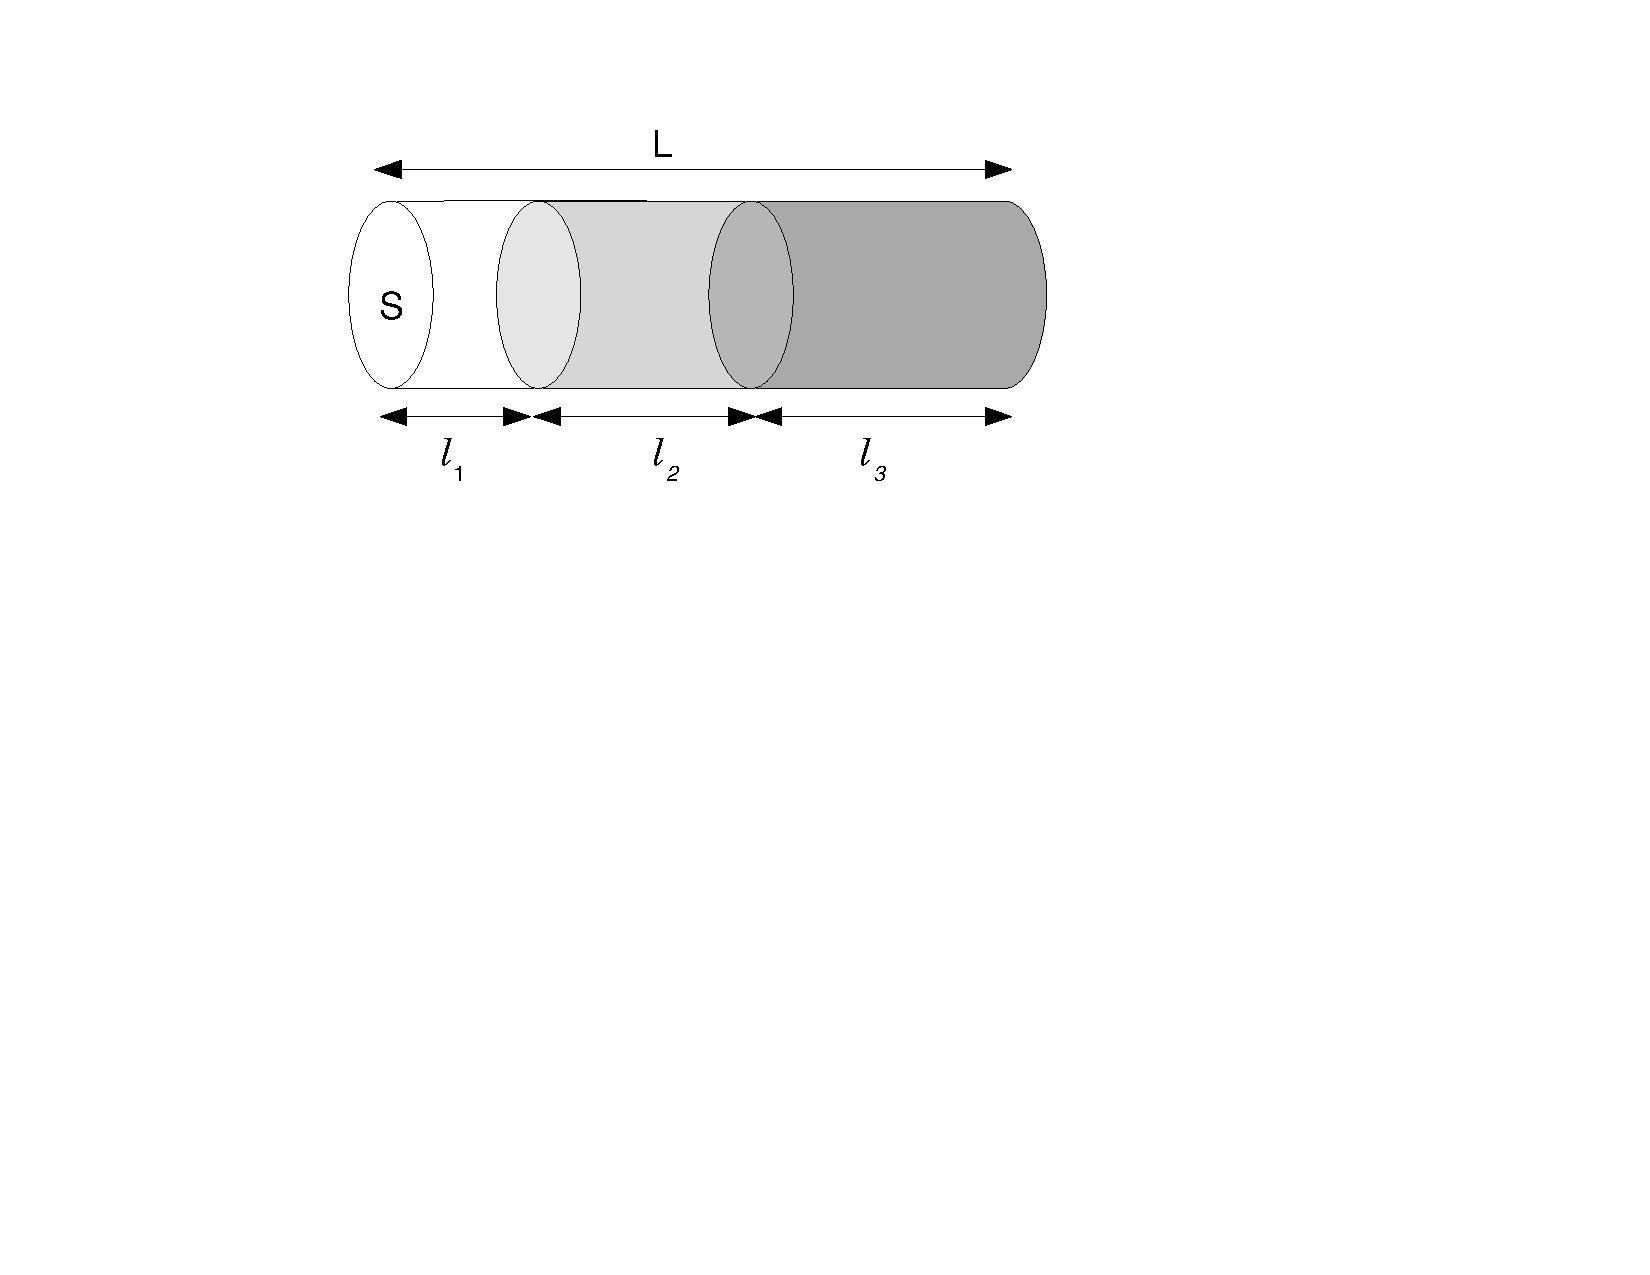
\includegraphics[width=0.4\textwidth]{fig/can.pdf}
\end{center}
\caption{Sketch of a simplified cylindrical volume made up of three different materials.}
\label{fig:can}
\end{figure}

The proposed method to investigate the impact on the detector performance of residual discrepancies $\DM$'s consists in changing in an appropriate and controlled way the material components by using a set of k-factors $\kvect\equiv(k_1, ..., k_i, ..., k_N)$ and then studying the effects on $\TX$ and $\TI$, e.g.:
\begin{equation}
\TX = \sum^N_i \rho_i \frac{\ell_i}{\Xo_i} \rightarrow  \TX_\kvect = \sum^N_i k_i \rho_i \frac{\ell_i}{\Xo_i},
\end{equation}
and
\begin{equation}
\TI = \sum^N_i \rho_i \frac{\ell_i}{\lI_i} \rightarrow  \TI_\kvect = \sum^N_i k_i \rho_i \frac{\ell_i}{\lI_i}.
\end{equation}

%\section{Parser}

The method described in the previous section can only be practically implemented by modifying the material densities in the DDD xml files describing the detector geometry. This is done by using a software tool written on purpose consisting of a perl xml parser. It takes the DDD material xml files in input and then, according to a {\em scenario} configuration file, changes the effective density of the material under study and of all materials that depend (directly and indirectly) on it; finally the modified xml files are written in output. These modified xml files are fully working in CMSSW.

%%%%%%%%%%%%%%%%%%%%%%%%%%%%%%%
%The detailed modification procedure is the following:
%\begin{enumerate}
%\item the density attribute is modified according to the k-factors in the tags {\tt <ElementaryMaterial .../>} or {\tt <CompositeMaterial .../>} where the materials are defined;
%\item all composite materials that depend on the modified materials are accordingly modified; if the composite material has density $\rho$ and fractions $w_j$, $j$ being the index running over the components, the parser apply the following substitutions:
%\begin{equation}
%w_j \to \frac{k_jw_j}{\sum kw}, \,\,\,\,\, \rho \to \rho \sum kw;
%\end{equation}
%\item step b) is repeated recursively with a scaling factor $1/\sum kw$ for all materials modified in the step b).
%\end{enumerate}
%
%The parser is accessible via CVS in ...
%
%The parser can be launched by using the wrapper script {\tt xmlFatThaMat.sh}:
%{\small
%\begin{Verbatim}[frame=leftline]
%./xmlSuperPorker.sh <scenario-file> <base-dir>
%\end{Verbatim}
%}
%where {\tt <scenario-file>} is the scenario configuration file described below and {\tt 
%<base-dir>} is the directory to which the paths of the xml files to be modified in the scenario file are referred. It is essentially the base dir of the CMSSW work area we are using.
%
%
%\subsection{The {\em scenario} configuration file}
%
%An example of the scenario configuration file is given below; it is the scenario file designed to properly change the Aluminium mass in the simulation; in  this case, for example, you want to skip materials that do contain Al (i.e.Alumina!) but that you want to study independently.
%
%{\small
%\begin{Verbatim}[frame=leftline]
%<?xml version="1.0"?>
%<scenario>
%<file name="./Geometry/TrackerCommonData/data/tecmaterial.xml" />
%<file name="./Geometry/TrackerCommonData/data/tibmaterial.xml" />
%<file name="./Geometry/TrackerCommonData/data/tibtidcommonmaterial.xml" />
%<file name="./Geometry/TrackerCommonData/data/tidmaterial.xml" />
%<file name="./Geometry/TrackerCommonData/data/tobmaterial.xml" />
%<file name="./Geometry/TrackerCommonData/data/trackermaterial.xml" />
%<file name="./Geometry/CMSCommonData/data/materials.xml" />
%<ElementaryMaterial name="Aluminium" kfactor="1.1">
%<SkipMaterial name="Ceramic"/>
%<SkipMaterial name="Alumina"/>
%<SkipMaterial name="Steel-008"/>
%<SkipMaterial name="Borosilicate_Glass"/>
%<SkipMaterial name="TEC_PitchAdapter"/>
%</ElementaryMaterial>
%</scenario>
%\end{Verbatim}
%}
%
%Each scenario file tag has its own meaning:
%\begin{itemize}
%\item the tags {\tt <file .../>} define the xml material files to be
%  altered; the material files not included in any tag are not changed;
%%- il tag <path .../> (sopra commentato) definisce un altro eventuale
%%  path comune, oltre a quello definito in linea di comando (base-dir)
%  che debba precedere il path di ciascun file;
%\item there are three possible tags to define the material variations:
%\begin{description}
%  \item[{\tt <ElementaryMaterial ... />}] to modify an elementary
%    material and recursively all composite material that directly or
%    indirectly depend on it; if the attribute {\tt
%      recurse} is given with the option {\tt false} ({\tt
%      recurse=false"}) the recursive modification is not done and the
%    modification is restricted to the pure elementary material only;
%  \item[{\tt <CompositeMaterial ... />}] to modify a composite
%    material and recursively all composite material that directly or 
%    indirectly depend on it; if the attribute {\tt
%      recurse} is given with the option {\tt false} ({\tt
%      recurse=''false"}) the recursive modification is not done and the
%    modification is restricted to the pure composite material only;
%  \item[{\tt <rMaterial ... />}] to modify all composite materials
%    that contain the specified {\tt rMaterial} and recursively all composite material that directly or 
%    indirectly depend on it; in this case the material name must
%    contain the namespace also; this tags is useful in the case a
%    given material needs to be modified but the file containing the
%    material definition is not included in any of the {\tt <file
%      .../>} tags. 
%\end{description}
%For all material modification tags the amount of alteration is
%defined via the attribute {\tt kfactor} ({\tt kfactor="..."}) that quantifies the
%multiplicative factor of the density change.
%
%All material modification tags also accept the following tags for
%extra functionalities:
%\begin{description}
%  \item[{\tt <SkipMaterial ... />}] to specify one or more {\tt CompositeMaterial} 
%  that has to remain unaltered;
%\item[{\tt <OnlyMaterial ... />}] to exclusively specify the {\tt CompositeMaterial} 
%  that has to be altered; if a tag of this kind is present
%  no other modification is done;
%\item[{\tt <SkipNamespace ... />}] to specify one or more namespaces,
%  i.e. files, that has to remain unaltered;
%\end{description}
%\end{itemize}
%
%As an output, the parser produces a modified xml file per each input
%file configured in the {\tt <file ... />} tags. The new file has the
%same name of the original one but the extension {\tt .xml} is changed
%into {\tt .xml.fat}. Within these output files, the modified materials
%are identified by the attribute {\tt fat="true"} in the corresponding
%material definition tags.
%
%\subsection{Helper scripts}
%
%To ease the material modification onto a typical CMSSW working area, two scripts have been written:
%CMSSW work area:
%\begin{description}
%\item[{\tt fat.sh}] (usage: {\tt ./fat.sh <scenario-file> <base-dir>})
%  make the parser modify the material files under the {\tt
%    <base-dir>} according to the given {\tt <scenario-file>}; the
%  original xml files are replaced by the modified ones in order to
%  have a working CMSSW area with the new material files; the old ones
%  are saved with the extension {\tt .xml.orig}; the replacement does
%  not occur in the case original files appear to be already treated by
%  the parser (i.e. the string {\tt fat="true"} is found in the input
%  files); this to avoid to apply material modification in cascade by mistake;
%\item[{\tt defat.sh}] (usage: {\tt ./defat.sh <base-dir>}) restores
%  the original xml files by using the saved versions. 
%\end{description}
%%%%%%%%%%%%%%%%%%%%%%%%%%%%%%%%%%%%%%%%%%%%%%

\section{The Tracker Recipe}

As  first application of the method, the Tracker
composition in the simulation was evaluated. GEANT4 tools, in fact, 
make easy to dump the total mass and the composition only in terms of
chemical elements of a given physical volume, and thus also of
the entire Tracker. More interesting is the understanding of the composition of
the Tracker in terms of basic materials, commonly encountered in the construction, e.g.:
\begin{itemize}
\item[-] pure chemical elements, as aluminium, copper, or silicon;
\item[-] simple compounds like alumina (${\rm Al}_2{\rm O}_3$) or glass;
\item[-] more complicated compounds like carbon fiber, FR4 or plastics. 
\end{itemize}
The total mass of the Tracker is \fixme
\begin{equation}
M({\rm Tracker}) = \sum_i m_i = \sum_i \rho_i V_i,
\end{equation}
where $i$ is the index running on the material components and $m_i$,
$\rho_i$ and $V_i$ are, respectively, the mass, the density, and the
volume of the component $i$.

To extract the contribution of a specific material $j$,
the method can be applied with the k-factor different from unity only
for the material under investigation. In this case the resulting total mass
of the entire Tracker volume becomes:
\begin{equation}
M_{\vec{k}=(..., 1, k_j, 1, ...)} (\mathrm{Tracker}) = M +
( k_j - 1) m_j,
\end{equation}
from which it is straightforward to derive the mass of the component $j$: 
\begin{equation}
m_j = \frac{M_{\vec{k}=(..., 1, k_j, 1, ...)} - M}{k_j
  - 1}.
\end{equation}
The procedure, repeated for all the material components, allows the Tracker composition to be derived. 
%The sum of the component masses estimated in this way is equal to the total Tracker mass within 1ppm. The exercise confirms that the method is correctly implemented
The composition of the whole Tracker is given in table~\ref{table:Tracker}: The sum of the component masses derived by this method agrees within 1 ppm with the total Tracker mass as directly given by GEANT4. This exercise is a confirmation that the method works and it is correctly implemented.

The composition of the individual subdetectors are reported in Appendix~\ref{compositionAppendix}.

\begin{table}[h]
\begin{center}
\begin{tabular}{clrrrrrr}
  &           & \multicolumn{2}{c}{Weight} & \multicolumn{2}{c}{Total} & \multicolumn{2}{c}{Remaining} \\ 
  & Name      & [kg]    & Fraction & [kg]  & Fraction & [kg]   & Fraction \\ 
 \hline 
 1 &          CarbonFiber & 1144.503 & 27.631\% & 1144.503 & 27.631\%  & 2997.524 & 72.369\% \\
 2 &               Copper & 595.674 & 14.381\% & 1740.176 & 42.013\%  & 2401.851 & 57.987\% \\
 3 &            Aluminium & 594.960 & 14.364\% & 2335.136 & 56.377\%  & 1806.891 & 43.623\% \\
 4 &                   PE & 354.633 & 8.562\% & 2689.769 & 64.938\%  & 1452.258 & 35.062\% \\
 5 &                C6F14 & 258.890 & 6.250\% & 2948.659 & 71.189\%  & 1193.368 & 28.811\% \\
 6 &              Silicon & 225.847 & 5.453\% & 3174.506 & 76.641\%  & 967.521 & 23.359\% \\
 7 &                Nomex & 123.331 & 2.978\% & 3297.836 & 79.619\%  & 844.190 & 20.381\% \\
 8 &                  G10 & 110.180 & 2.660\% & 3408.016 & 82.279\%  & 734.011 & 17.721\% \\
 9 &                  FR4 & 103.238 & 2.492\% & 3511.254 & 84.771\%  & 630.773 & 15.229\% \\
10 &              Ceramic &  91.062 & 2.198\% & 3602.316 & 86.970\%  & 539.711 & 13.030\% \\
11 &               Kapton &  82.757 & 1.998\% & 3685.073 & 88.968\%  & 456.954 & 11.032\% \\
12 &                Steel &  81.521 & 1.968\% & 3766.595 & 90.936\%  & 375.432 & 9.064\% \\
13 &                Epoxy &  57.053 & 1.377\% & 3823.647 & 92.313\%  & 318.380 & 7.687\% \\
14 &             Graphite &  50.237 & 1.213\% & 3873.884 & 93.526\%  & 268.143 & 6.474\% \\
15 &               Quartz &  39.025 & 0.942\% & 3912.909 & 94.468\%  & 229.118 & 5.532\% \\
16 &             Titanium &  31.707 & 0.765\% & 3944.615 & 95.234\%  & 197.412 & 4.766\% \\
17 &             Acrylate &  29.604 & 0.715\% & 3974.220 & 95.949\%  & 167.807 & 4.051\% \\
18 &    BorosilicateGlass &  23.134 & 0.559\% & 3997.354 & 96.507\%  & 144.673 & 3.493\% \\
19 &               Bronze &  19.910 & 0.481\% & 4017.264 & 96.988\%  & 124.763 & 3.012\% \\
20 &          SiliconeGel &  18.246 & 0.440\% & 4035.510 & 97.428\%  & 106.517 & 2.572\% \\
21 &               Silver &  16.053 & 0.388\% & 4051.562 & 97.816\%  &  90.465 & 2.184\% \\
22 &                Brass &  14.932 & 0.361\% & 4066.495 & 98.176\%  &  75.532 & 1.824\% \\
23 &             Rohacell &  14.539 & 0.351\% & 4081.034 & 98.527\%  &  60.993 & 1.473\% \\
24 &                 CuNi &  13.941 & 0.337\% & 4094.975 & 98.864\%  &  47.052 & 1.136\% \\
25 &              Solders &   9.868 & 0.238\% & 4104.842 & 99.102\%  &  37.184 & 0.898\% \\
26 &                 BaTi &   9.837 & 0.237\% & 4114.680 & 99.340\%  &  27.347 & 0.660\% \\
27 &           Inconel600 &   7.426 & 0.179\% & 4122.105 & 99.519\%  &  19.922 & 0.481\% \\
28 &               Kevlar &   5.119 & 0.124\% & 4127.224 & 99.643\%  &  14.803 & 0.357\% \\
29 &        SiliconNoSens &   4.161 & 0.100\% & 4131.385 & 99.743\%  &  10.642 & 0.257\% \\
30 &                 Iron &   3.919 & 0.095\% & 4135.305 & 99.838\%  &   6.722 & 0.162\% \\
31 &                 Peek &   3.572 & 0.086\% & 4138.877 & 99.924\%  &   3.150 & 0.076\% \\
32 &               Nickel &   1.675 & 0.040\% & 4140.552 & 99.964\%  &   1.475 & 0.036\% \\
33 &            Beryllium &   0.760 & 0.018\% & 4141.311 & 99.983\%  &   0.716 & 0.017\% \\
34 &                 Gold &   0.525 & 0.013\% & 4141.836 & 99.995\%  &   0.191 & 0.005\% \\
35 &            Resistors &   0.172 & 0.004\% & 4142.008 & 100.000\%  &   0.019 & 0.000\% \\
36 &                  Air &   0.019 & 0.000\% & 4142.027 & 100.000\%  &   0.000 & 0.000\% \\
 \hline 
  & Total & 4142.027 & 100.000\% & & & & \\ 

\end{tabular}
\caption{Mass of the basic components in the Tracker volume.}
\label{table:Tracker}
\end{center}
\end{table}

\clearpage 

\section{The $\TX$ and $\TI$ dependence on materials}

%\subsection{Material classification in categories}

Although the perl xml parser can deal with each of the 37 \fixme  basic materials listed in table~\ref{table:Tracker},
for the following analysis these basic materials were grouped into a limited number of {\it categories} defined as a class of homogeneous and/or similar materials. A category can consist of just one basic material.
The category definitions are given in table~\ref{table:cat}.

\begin{table}[h]
\begin{center}
\begin{tabular}{clll}
  & Category    & Short       &           \\ 
  & Name        & Name        & Components \\
  \hline 
  1 & CarbonFiber & CarbonFiber & CarbonFiber \\
  \hline 
  2 & Other mechanical structure & OtherMechStruct & Nomex \\
  & &             & Graphite \\
  & &            & Rohacell \\
  & &             & Peek   \\
  \hline 
  3 & Copper and copper alloys & CopperAndCuAlloys & Copper \\
  & & &              Bronze \\
  & & &                 Brass \\
  & & &           CuNi \\
  \hline 
  4 & Aluminium & Aluminium & Aluminium \\ 
  \hline 
  5 & Organic materials & OrganicMaterials & PE \\
  & & &               Kapton \\
  & & &       Acrylate \\
  & & &  Kevlar \\
  \hline 
6 & C6F14 & C6F14 & C6F14 \\
  \hline 
7 & Silicon sensitive & Silicon & Silicon \\
  \hline 
8 & Fiber Glass laminated & FiberGlassLaminated & FR4 \\
& & &                  G10 \\
  \hline 
9 & Inorganic oxides & InorganicOxides & Ceramic \\
& & &               Quartz \\
& & &    BorosilicateGlass \\
  \hline 
10 & Other metals & OtherMetals &  Steel \\
& & &             Titanium \\
 & & &              Silver \\
  & & &         Inconel600 \\
 & & &                Iron \\
 & & &           Beryllium \\
 & & &                Gold \\
  \hline 
11 & Glue and resins & GlueAndResins &  Epoxy \\
& & &        SiliconeGel \\
  \hline 
12 & Electronic components & ElectronicComponents & Solders \\
& & &                  BaTi \\
& & &         SiliconNoSens \\
& & &                Nickel \\
& & &             Resistors \\
  \hline 
13 & Air & Air & Air \\
\end{tabular}
\caption{Table of definitions of material categories.}
\label{table:cat}
\end{center}
\end{table}

The contributions of each of the above categories to the whole Tracker mass are listed in table~\ref{table:TrackerCat} 
and illustrated in the top plot of figure~\ref{fig:summaryMaterials}.
Details for the individual subdetector volumes are reported in Appendix~\ref{categoriesAppendix}.
\begin{table}[h]
\begin{center}
\begin{tabular}{clrrrrrr}
  &           & \multicolumn{2}{c}{Mass} & \multicolumn{2}{c}{Total} & \multicolumn{2}{c}{Remaining} \\ 
  & Name      & [kg]    & Fraction & [kg]  & Fraction & [kg]   & Fraction \\ 
 \hline 
 1 &          CarbonFiber & 1144.503 & 27.631\% & 1144.503 & 27.631\%  & 2997.524 & 72.369\% \\
 2 &    CopperAndCuAlloys & 644.458 & 15.559\% & 1788.960 & 43.190\%  & 2353.067 & 56.810\% \\
 3 &            Aluminium & 594.960 & 14.364\% & 2383.920 & 57.554\%  & 1758.107 & 42.446\% \\
 4 &     OrganicMaterials & 472.113 & 11.398\% & 2856.033 & 68.953\%  & 1285.994 & 31.047\% \\
 5 &                C6F14 & 258.890 & 6.250\% & 3114.923 & 75.203\%  & 1027.104 & 24.797\% \\
 6 &              SiliconSensitive & 225.847 & 5.453\% & 3340.770 & 80.655\%  & 801.257 & 19.345\% \\
 7 &  FiberGlassLaminated & 213.418 & 5.152\% & 3554.188 & 85.808\%  & 587.839 & 14.192\% \\
 8 &      OtherMechStruct & 191.679 & 4.628\% & 3745.866 & 90.436\%  & 396.161 & 9.564\% \\
 9 &      InorganicOxides & 153.221 & 3.699\% & 3899.087 & 94.135\%  & 242.940 & 5.865\% \\
10 &          OtherMetals & 141.909 & 3.426\% & 4040.997 & 97.561\%  & 101.030 & 2.439\% \\
11 &        GlueAndResins &  75.298 & 1.818\% & 4116.295 & 99.379\%  &  25.732 & 0.621\% \\
12 & ElectronicComponents &  25.713 & 0.621\% & 4142.008 & 100.000\%  &   0.019 & 0.000\% \\
13 &                  Air &   0.019 & 0.000\% & 4142.027 & 100.000\%  &   0.000 & 0.000\% \\
 \hline 
  & Total & 4142.027 & 100.000\% & & & & \\ 

\end{tabular}
\caption{Mass per material category in the Tracker volume.}
\label{table:TrackerCat}
\end{center}
\end{table}
%%

The dependence of $\TX$ and $\TI$ on the single category contribution is the starting point of the systematic study. These dependences are also very important to understand which category dominates the total radiation length and which category is, on the other hand, negligible.The derivation of the dependence of $\TX$ and $\TI$ on the categories is similar to the method described above for the mass fractions.
For example for the thickness in units of radiation length $\TX$, if $k_j$ is the factor different from unity
\begin{equation}
\mathrm{\TX}_{(...,1,{k_j},1...)} = \mathrm{\TX} + (k_j - 1) t_{{\rm R}j},
\end{equation}
from which it is straightforward to derive the respective component $t_{Rj}$:
\begin{equation}
t_{{\rm R}j} = \frac{\mathrm{\TX}_{(...,1,k_j,1...)} - \mathrm{\TX}}{k_j - 1} .
\end{equation}
The contributions of each of the above categories to the $\TX$ and $\TI$, averaged on the overall Tracker volume, 
are illustrated in the middle and bottom plots of figure~\ref{fig:summaryMaterials} respectively.
Figure~\ref{fig:x0Materials} shows the $\eta$ distributions of $\TX$ for the four categories mostly contributing
to the Tracker mass, while the distributions of $\TI$ as a function of $\eta$ for the same categories are shown in figure~\ref{fig:lambda0Materials}.
\begin{figure}[h]
\begin{center}
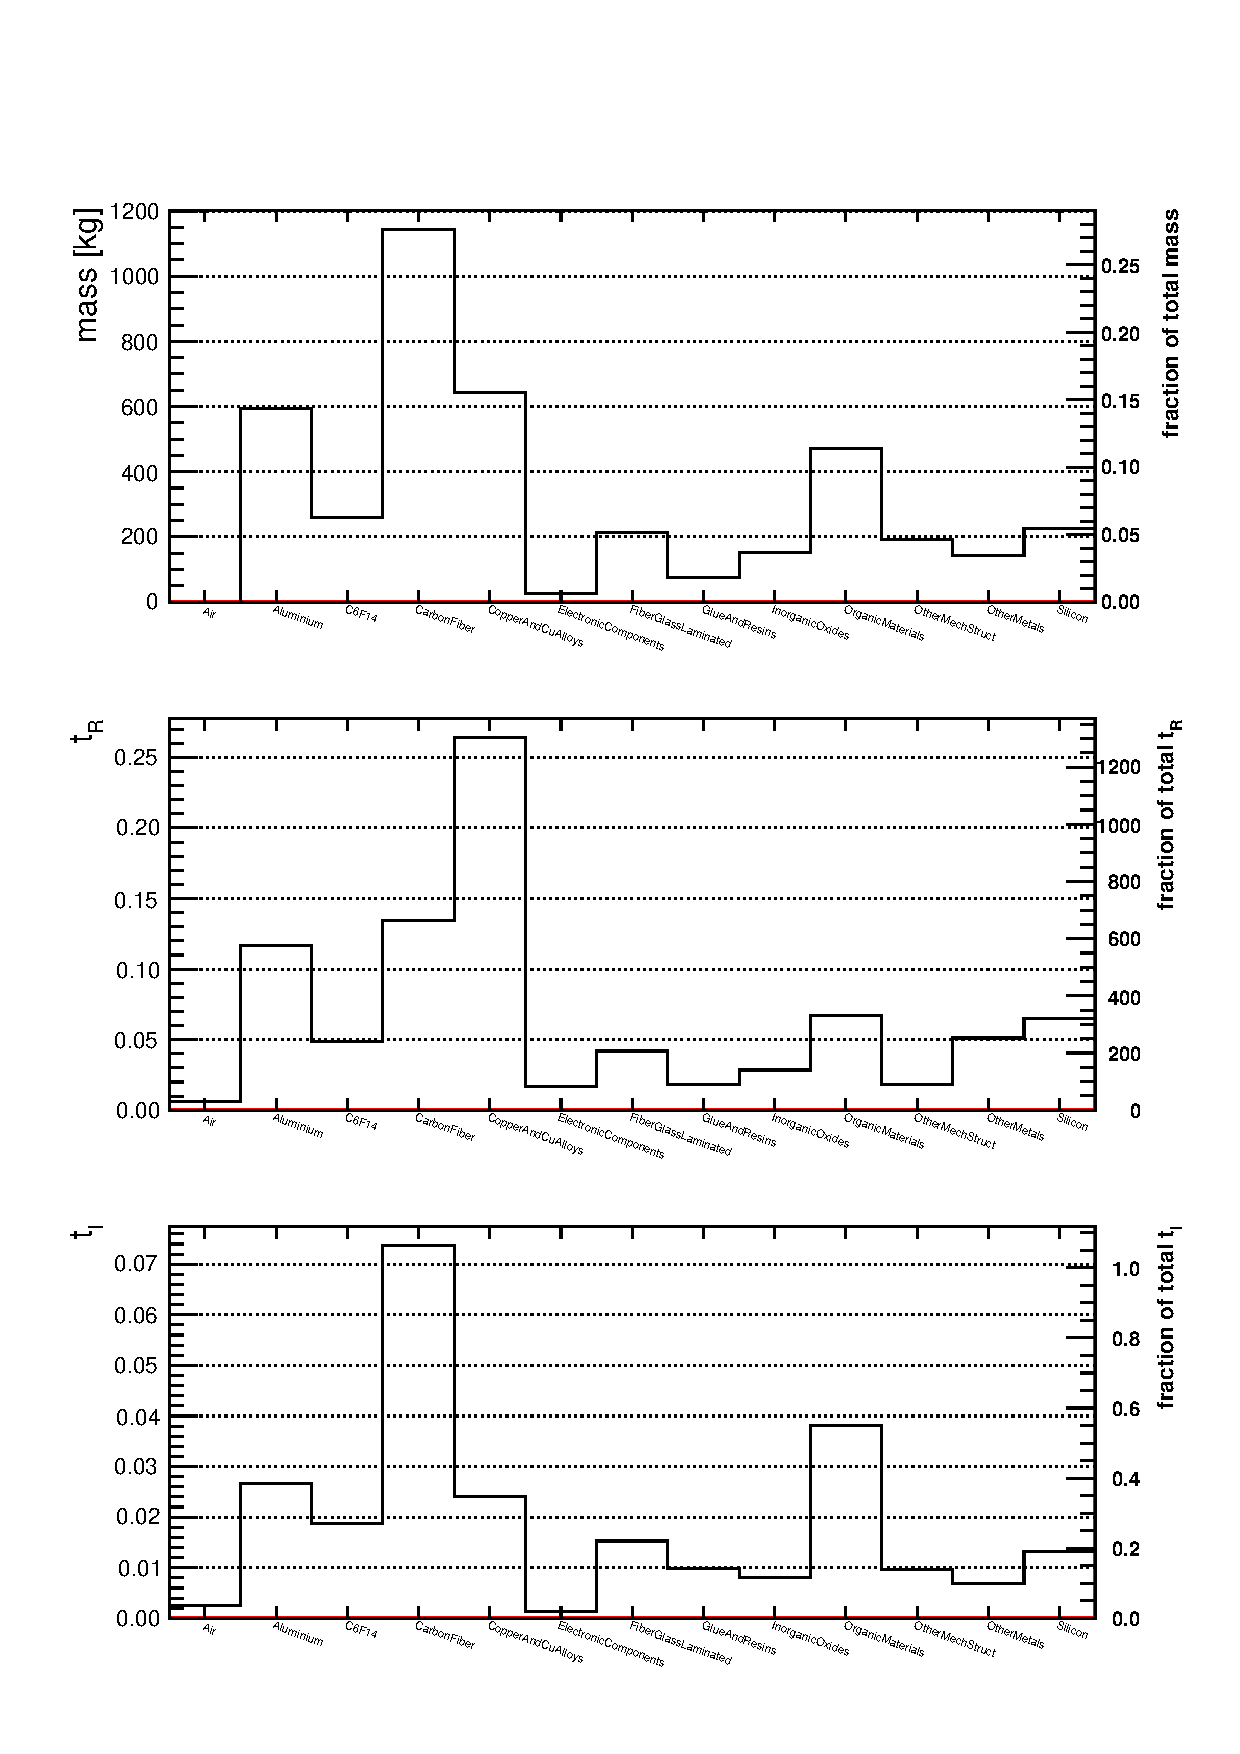
\includegraphics[width=\textwidth]{fig/SummaryMaterials.pdf}
\end{center}
\caption{Contribution of the categories listed in table~\ref{table:cat} to the total mass of the Tracker (top), average $\TX$ (center) and average $\TI$ (bottom). 
Values on the left vertical axis indicates absolute contributions while relative contributions are indicated on the right.}
\label{fig:summaryMaterials}
\end{figure}

\begin{figure}[th]
\begin{center}
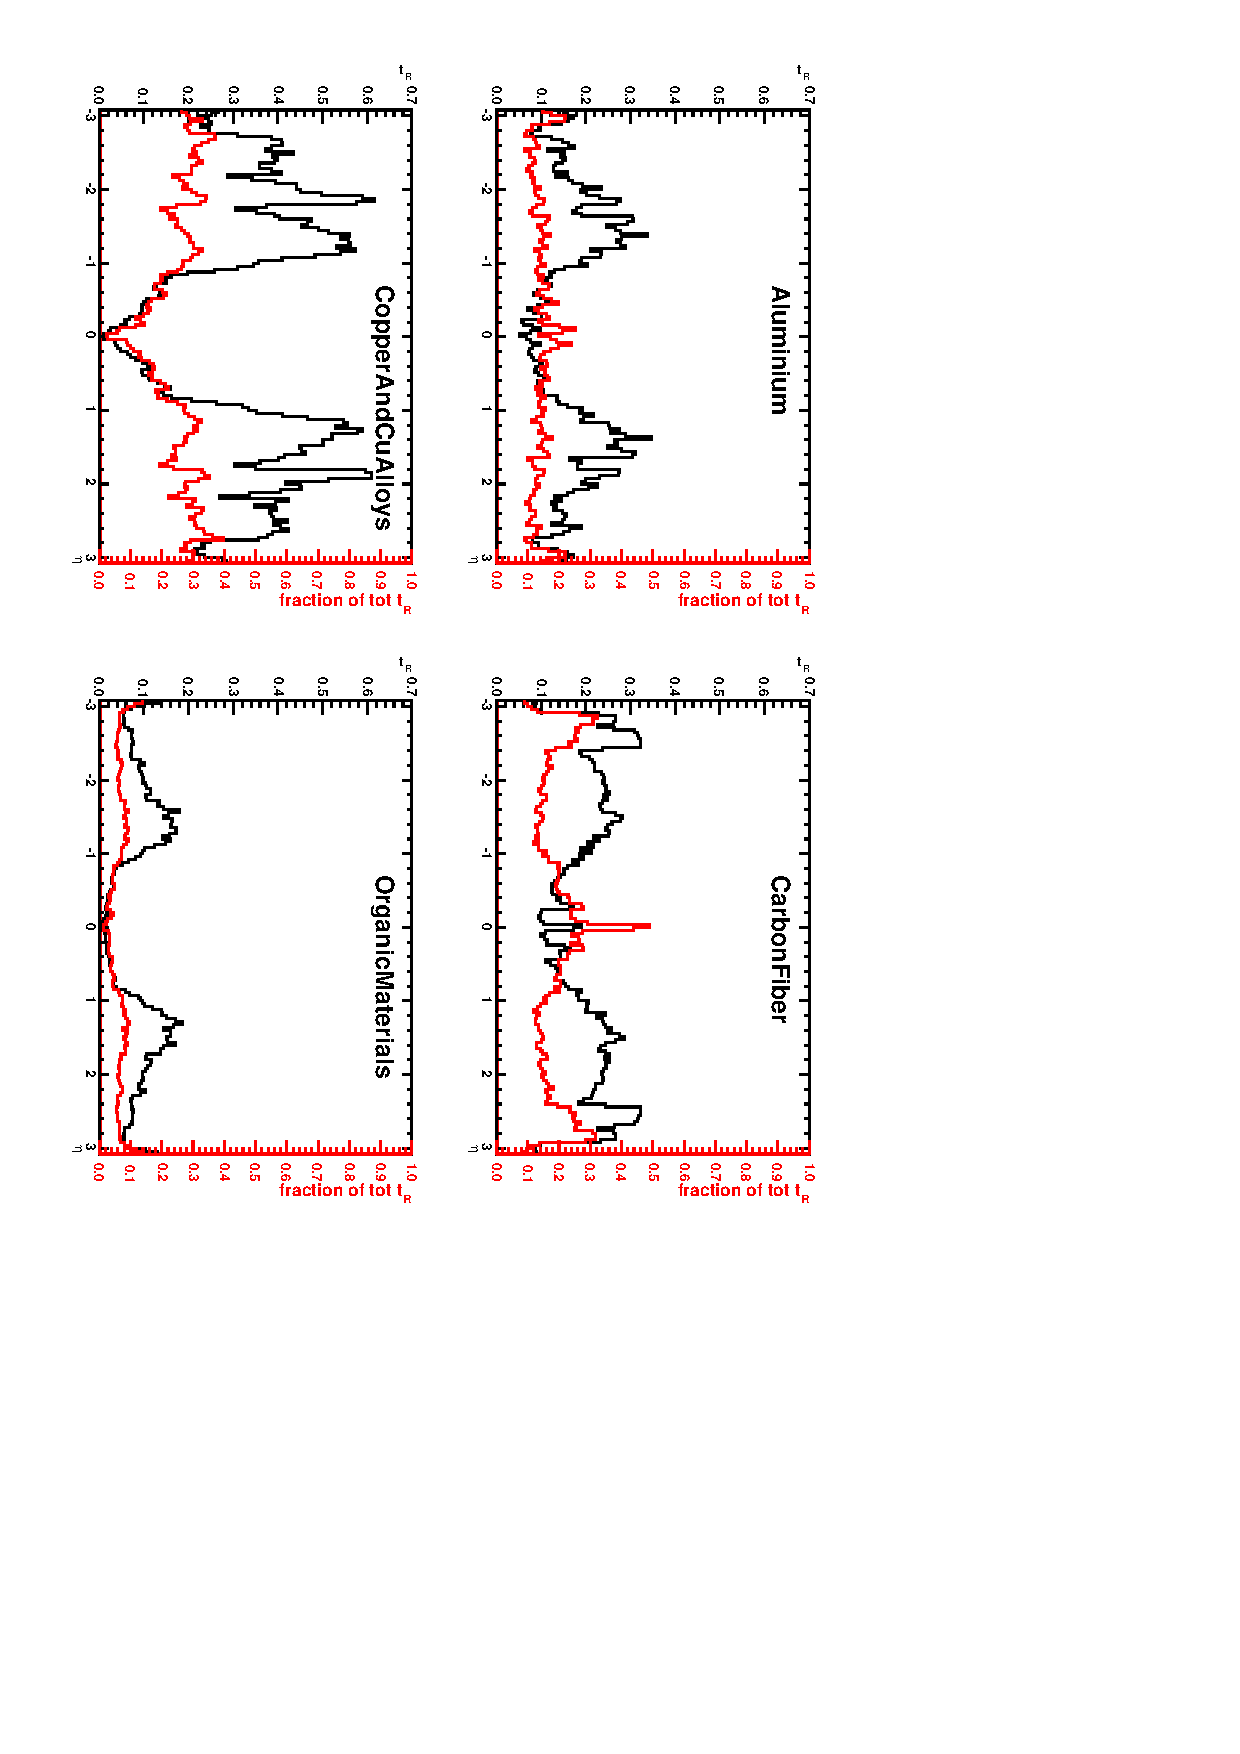
\includegraphics[width=0.7\textwidth,angle=90]{fig/x0Materials.pdf}
\end{center}
\caption{Distribution of the average thickness in units of radiation length $\Xo$ as a function of $\eta$ for the four categories of table~\ref{table:cat} mostly contributing to the total mass of the 
Tracker. 
Values on the left vertical axis indicates absolute contributions while relative contributions are indicated on the right.}
\label{fig:x0Materials}
\end{figure}

\begin{figure}[bh]
\begin{center}
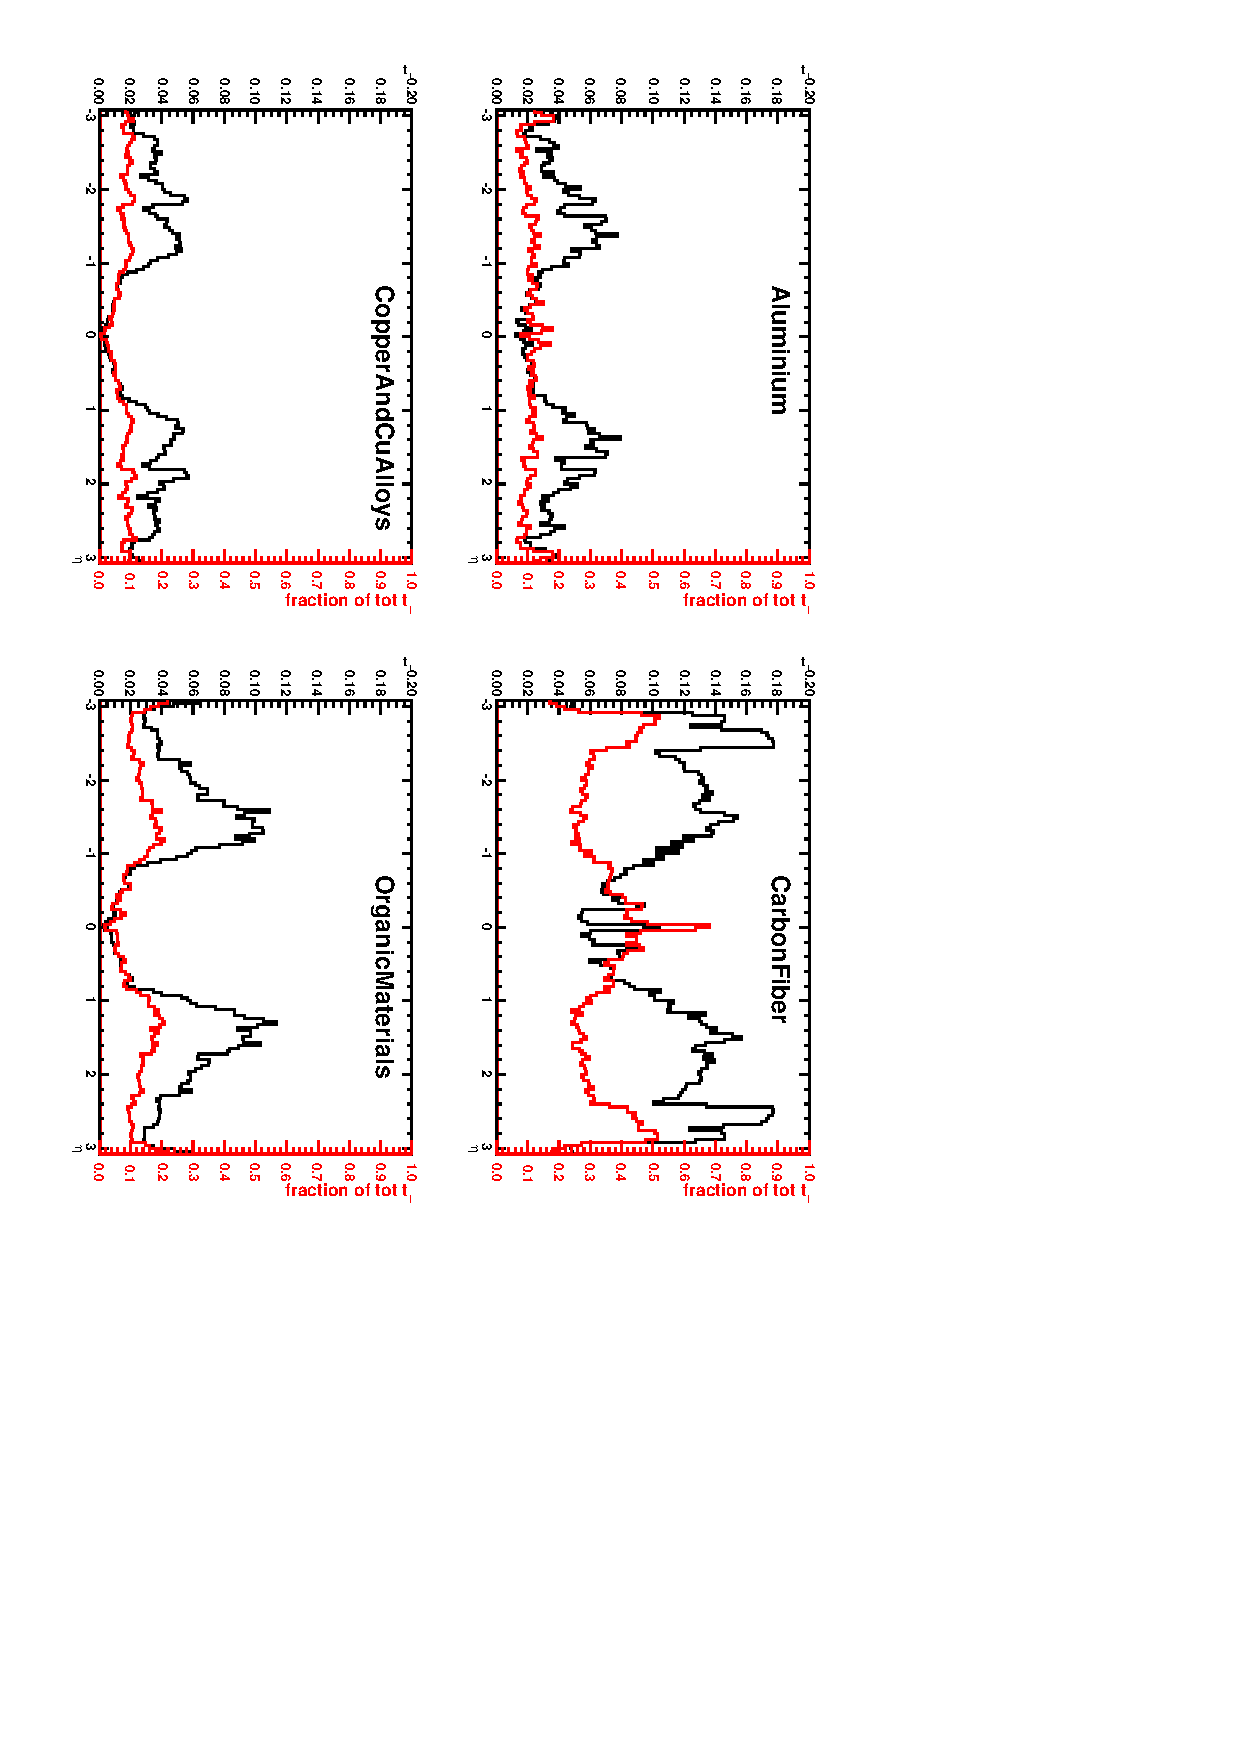
\includegraphics[width=0.7\textwidth,angle=90]{fig/lambda0Materials.pdf}
\end{center}
\caption{Distribution of the average thickness in units of interaction length $\lI$ as a function of $\eta$ for the four categories of table~\ref{table:cat} mostly contributing to the total mass of the 
Tracker. 
Values on the left vertical axis indicates absolute contributions while relative contributions are indicated on the right.}
\label{fig:lambda0Materials}
\end{figure}


\section{Determination of the altered scenarios for the material budget}

The systematic uncertainties on the representation of the material at the level of GEANT4 simulation can be due several sources, as, for example, the lack of knowledge or approximation in the shape and size of the volumes, chemical compositions and mass. Independently of the source, any effect can be represented to the extent of our needs as an appropriate fractional changes $\nicefrac{\Delta \rho_i}{\rho_i}$ on the material densities, resulting in a variation on the total thickness
\begin{equation}
\Delta \mathrm{T} = \sum_i \frac{\Delta \rho_i}{\rho_i} t_i
\end{equation}
where, again, $\mathrm{T}$ can be $\TX$ or $\TI$ and $t_i$ the respective component determined by means of the method described above.

An insight on the systematic uncertainties on the knowledge of the material can be derived by maximizing or minimizing $\TX$ and $\TI$ with respect to the possible density variations within an allowed domain:
\begin{equation}
\mathrm{\TX} + \Delta \mathrm{\TX} = \sum_i \frac{\ell_i}{X_{0 i}} \left( \rho_i + \Delta \rho_i \right) = \sum_i \tX_i k_i,
\end{equation}
\begin{equation}
\mathrm{\TI} + \Delta \mathrm{\TI} = \sum_i \frac{\ell_i}{\lambda_{{\mathrm I} i}} \left( \rho_i + \Delta \rho_i \right) = \sum_i \tI_i k_i.
\end{equation}

The aim of the present study is to derive the set of k-factors $\kvect^{\rm R}_{\rm min}$ ({\em minimal $X_0$ scenario}) and $\kvect^{\rm R}_{\rm max}$ ({\em maximal $X_0$ scenario})  corresponding to the minimal and maximal variations $\Delta \TX_{\rm min}$ and $\Delta \TX_{\rm max}$ compatible with the systematic uncertainties. Similar entities can be defined with respect to $\lambda_{\rm I}$ in place of $X_0$: $\kvect^{\rm I}_{\rm min}$ ({\em minimal $\lambda_{\rm I}$ scenario}) and $\kvect^{\rm I}_{\rm max}$ ({\em maximal $\lambda_{\rm I}$ scenario}) corresponding to the minimal and maximal variations $\Delta \TI_{\rm min}$ and $\Delta \TI_{\rm max}$. The variation is defined as the average of $\Delta \TX$ or $\Delta \TI$ over the $\eta$ range comprised between $-3$ and $3$. 

The derivation of the maximal and minimal scenarios results from an extrema finding problem with respect to the variation of material densities intended to represent the effects of the systematic uncertainties. To ease the optimization procedure, the material categories are used in place of the basic materials, much larger in number. The approach is sound since similar materials have been grouped on purpose into homogeneous categories.

The density variation domain results by the imposition of an appropriate set of constraints. These are listed below.
\begin{itemize}
%
% http://indico.cern.ch/getFile.py/access?contribId=6&resId=0&materialId=slides&confId=26422
\item The overall difference between weighted mass and total simulated mass is kept fixed by imposing
 \begin{equation}
\Delta M = \sum_i \frac{\Delta \rho_i}{\rho_i} m_i.
\end{equation}
The Silicon Strip Tracker mass as estimated during the integration and installation is 3996$^{+88}_{-132}$ kg the Pixel detector, installed in a later time, is not included in this estimation; the corresponding mass in the simulation is 4037 kg. The resulting relative weighted versus simulated mass difference is $-1^{+2}_{-3}\%$ suggesting an agreement between weighted and simulated masses within the estimation error.


Similar estimation performed over single subdetector indicate possible localized larger discrepancies. For example the TIB/TID subdetector plus some ancillary pieces have been weighted. The result is 450$^{+12}_{-20}$ kg to be compared with 427.0 kg  the simulated mass of the corresponding volumes. The resulting weighted versus simulated mass difference is $5^{+3}_{-4}\%$. As far as the TEC subdetector is concerned an uncertainty of about $\sim 3\%$ is claimed by the experts.

As a consequence a conservative approach has been chosen in this study: it is assumed that the actual Tracker mass is $5\%$ larger than the mass on the corresponding volumes in the simulation. {\bf FIXME FIXME FIXME}
\item The density variation ranges within each category are constrained depending on the characteristic and typical use of the materials contained in the categories. A large amount of direct experience in integrating and assembling the Tracker is used in defining these numbers. They are listed in table~\ref{table:catVariations}.

Composite materials for which the chemical composition can vary substantially and used in shapes with not well defined geometry that can be difficult to represent in the simulation can vary up to $\pm 15\%$; typical examples in this typology is the carbon fiber and the organic material (i.e. plastics).

Pure materials and metals are typically well known chemically and easier to represent. The cooling fluid is an exception since its amount is estimated by the internal volume of the pipes that build up the cooling system, often with shapes very complicated. This estimation is difficult.

The category ``Glue and resins'' is assigned with a variation range as large as $\pm 20\%$ because volumes of glues, resins, silicone gel heavily used for assemblying modules and in the integration activity in general were not at all controlled with respect to the amounts used, very dependent of many parameters like temperature.

The density of the sensitive Silicon volume is kept fixed to avoid affecting the signal generated in the active volumes. Nevertheless it is worth noticing that also silicon detector thicknesses can vary up to $\sim 10\%$.
\end{itemize} 



\begin{table}[h]
\begin{center}
\begin{tabular}{clc}
  & Category    & Allowed density \\ 
  & Name        & Variation in $\%$    \\
  \hline 
  1 & Carbon Fiber               & $\pm15$ \\
  2 & Other mechanical structure & $\pm15$ \\
  3 & Copper and copper alloys   & $\pm5$ \\
  4 & Aluminium                   & $\pm5$\\ 
  5 & Organic materials          & $\pm15$ \\
  6 & C6F14                      & $\pm10$\\
  7 & Silicon sensitive          & Fixed                       \\
  8 & Fiber Glass laminated      & $\pm10$\\
  9 & Inorganic oxides           & $\pm5$ \\
 10 & Other metals               & $\pm10$\\
 11 & Glue and resins            & $\pm20$\\
 12 & Electronic components      & $\pm10$\\
 13 & Air                        & Fixed \\
\end{tabular}
\caption{Allowed density variation of the various material categories in the minimization/maximization problem.}
\label{table:catVariations}
\end{center}
\end{table}

\subsection{The extrema finding problem}

The determination of the k-factors was done with a
standard technique used for solving optimization problems with inequality
constraints, the so-called penalty function method. This method
consists in defining as  objective function the sum of the actual
function $f(x)$ to be minimized and a term penalizing the
objective whenever the constraint $g(x)\le 0$ is violated. 
The minimization of the objective function is then performed
iteratively, at every iteration starting from the value of $x$ found
in the previous step and progressively increasing the penalty term.

Here, the objective functions to be minimized were defined as: 
\begin{eqnarray*}
\TX(\kvect^{\rm R}) = \sum^N_i k_i t_{{\rm R}j} +
\epsilon^{\rm R}_r \left[ \left(\sum^N_i (k_i-1.05) \rho_i V_i\right)^2  + \sum^N_i
  g(k_i)^2 \right] \quad \text{for determining $\kvect^{\rm R}_{\rm min}$,}\\
\TX(\kvect^{\rm R}) = -\sum^N_i k_i t_{{\rm R}j}, +
\epsilon^{\rm R}_r \left[ \left(\sum^N_i (k_i-1.05) \rho_i V_i\right)^2  + \sum^N_i
  g(k_i)^2 \right] \quad \text{for determining $\kvect^{\rm R}_{\rm max}$,}\\
\TI(\kvect^{\rm I}) = \sum^N_i k_i t_{{\rm I}j} +
\epsilon^{\rm I}_r \left[ \left(\sum^N_i (k_i-1.05) \rho_i V_i\right)^2  + \sum^N_i
  g(k_i)^2 \right] \quad \text{for determining $\kvect^{\rm I}_{\rm min}$,}\\
\TI(\kvect^{\rm I}) = -\sum^N_i k_i t_{{\rm I},} +
\epsilon^{\rm I}_r \left[ \left(\sum^N_i (k_i-1.05) \rho_i V_i\right)^2  + \sum^N_i
  g(k_i)^2 \right] \quad \text{for determining $\kvect^{\rm I}_{\rm max}$.}
\end{eqnarray*}

In the above relations, the first term is the thickness to be
minimized, the second term represents the constraint on the change of
the total mass of the Tracker, and the last term the constraint from the
allowed range of variations of the k-factor of the category $i$
defined in table~\ref{table:catVariations}, e.g. $k_{i,min}\le  k_i\le
k_{i,max}$ where the constraint inequality are defined by the function:
\[
g(k_i)=
\begin{cases}
k_i-k_{i,min}&  \text{if $k_i<k_{i,min}$,} \\
k_{i,max}-k_i,&  \text{if $k_i>k_{i,max}$,} \\
0 & \text{otherwise.}
\end{cases}
\]
The evolution of the penalty functions are given by 
$\epsilon_r^{\rm R}=2^r$  and $\epsilon_r^{\rm I}=2^{r-1}$, with $r$
being the iteration number, defined to give 
contributions to the objective function of the same order of the
actual function to be minimized during the first iterations. A minimum satisfying the
constraints is reached in about ten iterations.

\begin{table}[h]
\begin{center}
\begin{tabular}{lcccc}
   Category    & $\kvect^{\rm R}_{max}$ &  $\kvect^{\rm R}_{min}$ &  $\kvect^{\rm I}_{max}$ &  $\kvect^{\rm I}_{min}$ 
\\ 
  \hline 
CarbonFiber             &  1.140  & 1.150  & 1.150 & 1.007 \\
OtherMechStruct         &  0.850  & 1.150  & 0.862 & 1.150 \\
CopperAndCuAlloys       &  1.050  & 0.950  & 0.950 & 1.050 \\           
Aluminium               &  1.050  & 1.004  & 0.950 & 1.050 \\           
OrganicMaterials        &  0.850  & 1.150  & 1.150 & 1.150 \\
C6F14                   &  1.100  & 1.100  & 1.100 & 1.100 \\
Silicon                 &  Fixed  & Fixed  & Fixed & Fixed \\
InorganicOxides         &  1.050  & 0.950  & 1.049 & 1.050 \\           
FiberGlassLaminated     &  1.100  & 0.902  & 1.100 & 1.013 \\   
OtherMetals             &  1.100  & 0.900  & 0.900 & 1.100 \\   
GlueAndResins           &  1.200  & 0.800  & 1.200 & 0.800 \\
ElectronicComponents    &  1.100  & 0.900  & 0.900 & 1.100 \\           
Air                     &  Fixed  & Fixed  & Fixed & Fixed \\
\hline
$\TX$ (default 1.184$\pm$0.002)    &1.249   &1.201  &  1.211  & 1.238 \\
$\TI$ (default 0.3495$\pm$0.0006)  &0.3683  &0.3705 &  0.3751 & 0.3645\\

\end{tabular}
\caption{Allowed density variation of the various material categories in the minimization/maximization problem.}
\label{table:catVariationsMinMax}
\end{center}
\end{table}

The average $\TX$ and $\TI$ for the four extrema scenarios are 
listed in table~\ref{table:catVariationsMinMax} and the fractional
changes in  the $\eta$  distributions are shown in figures~\ref{fig:x0minmax}
and~\ref{fig:lambda0minmax}. 


\begin{figure}[th]
\begin{center}
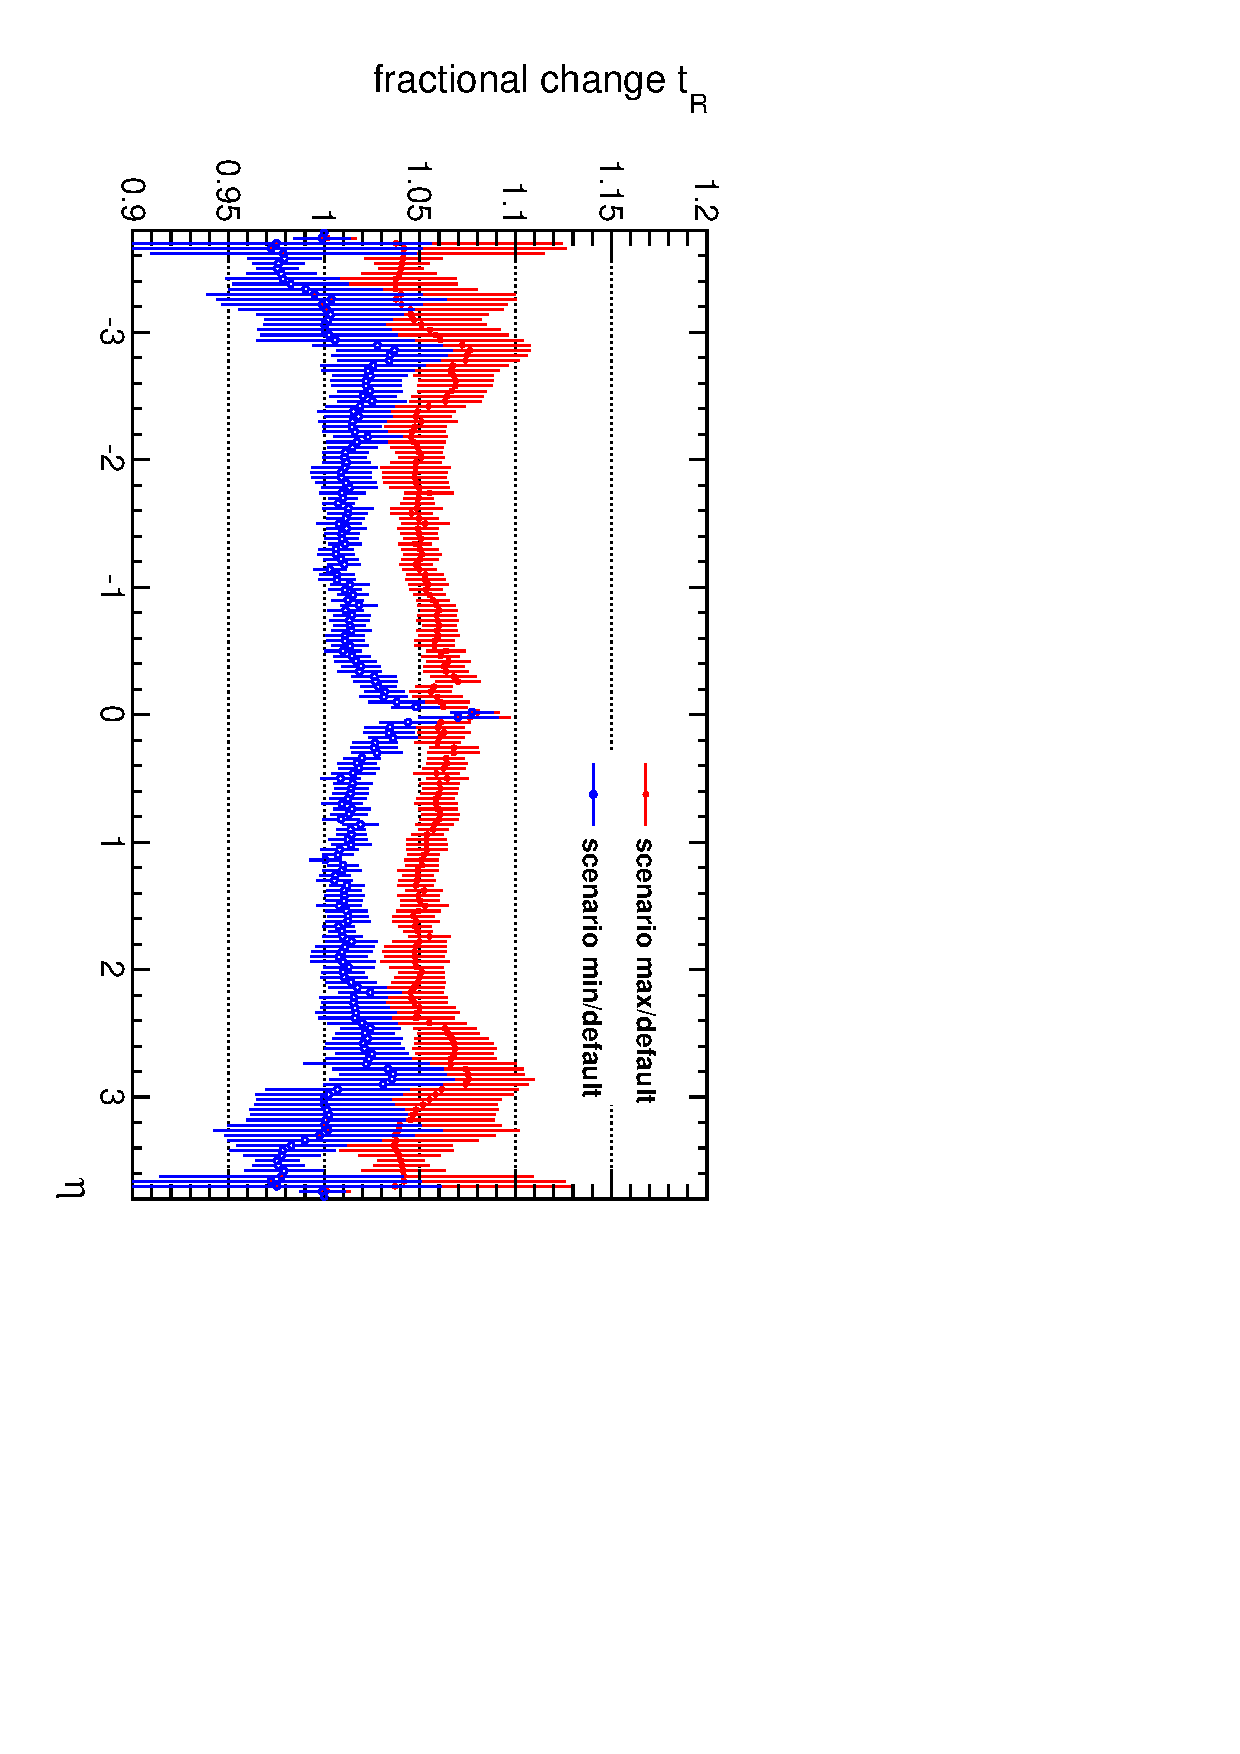
\includegraphics[width=0.5\textwidth,angle=90]{fig/x0minmax.pdf}
\end{center}
\caption{Fractional change of $\TX$ with respect the CMSSW setting
  for the $\kvect^{\rm R}_{max}$ and $\kvect^{\rm R}_{min}$ scenarios.
  An uniform increase of the Tracker mass of 5\% would correspond
  to a horizontal line at 1.05.}
\label{fig:x0minmax}
\end{figure}

\begin{figure}[bh]
\begin{center}
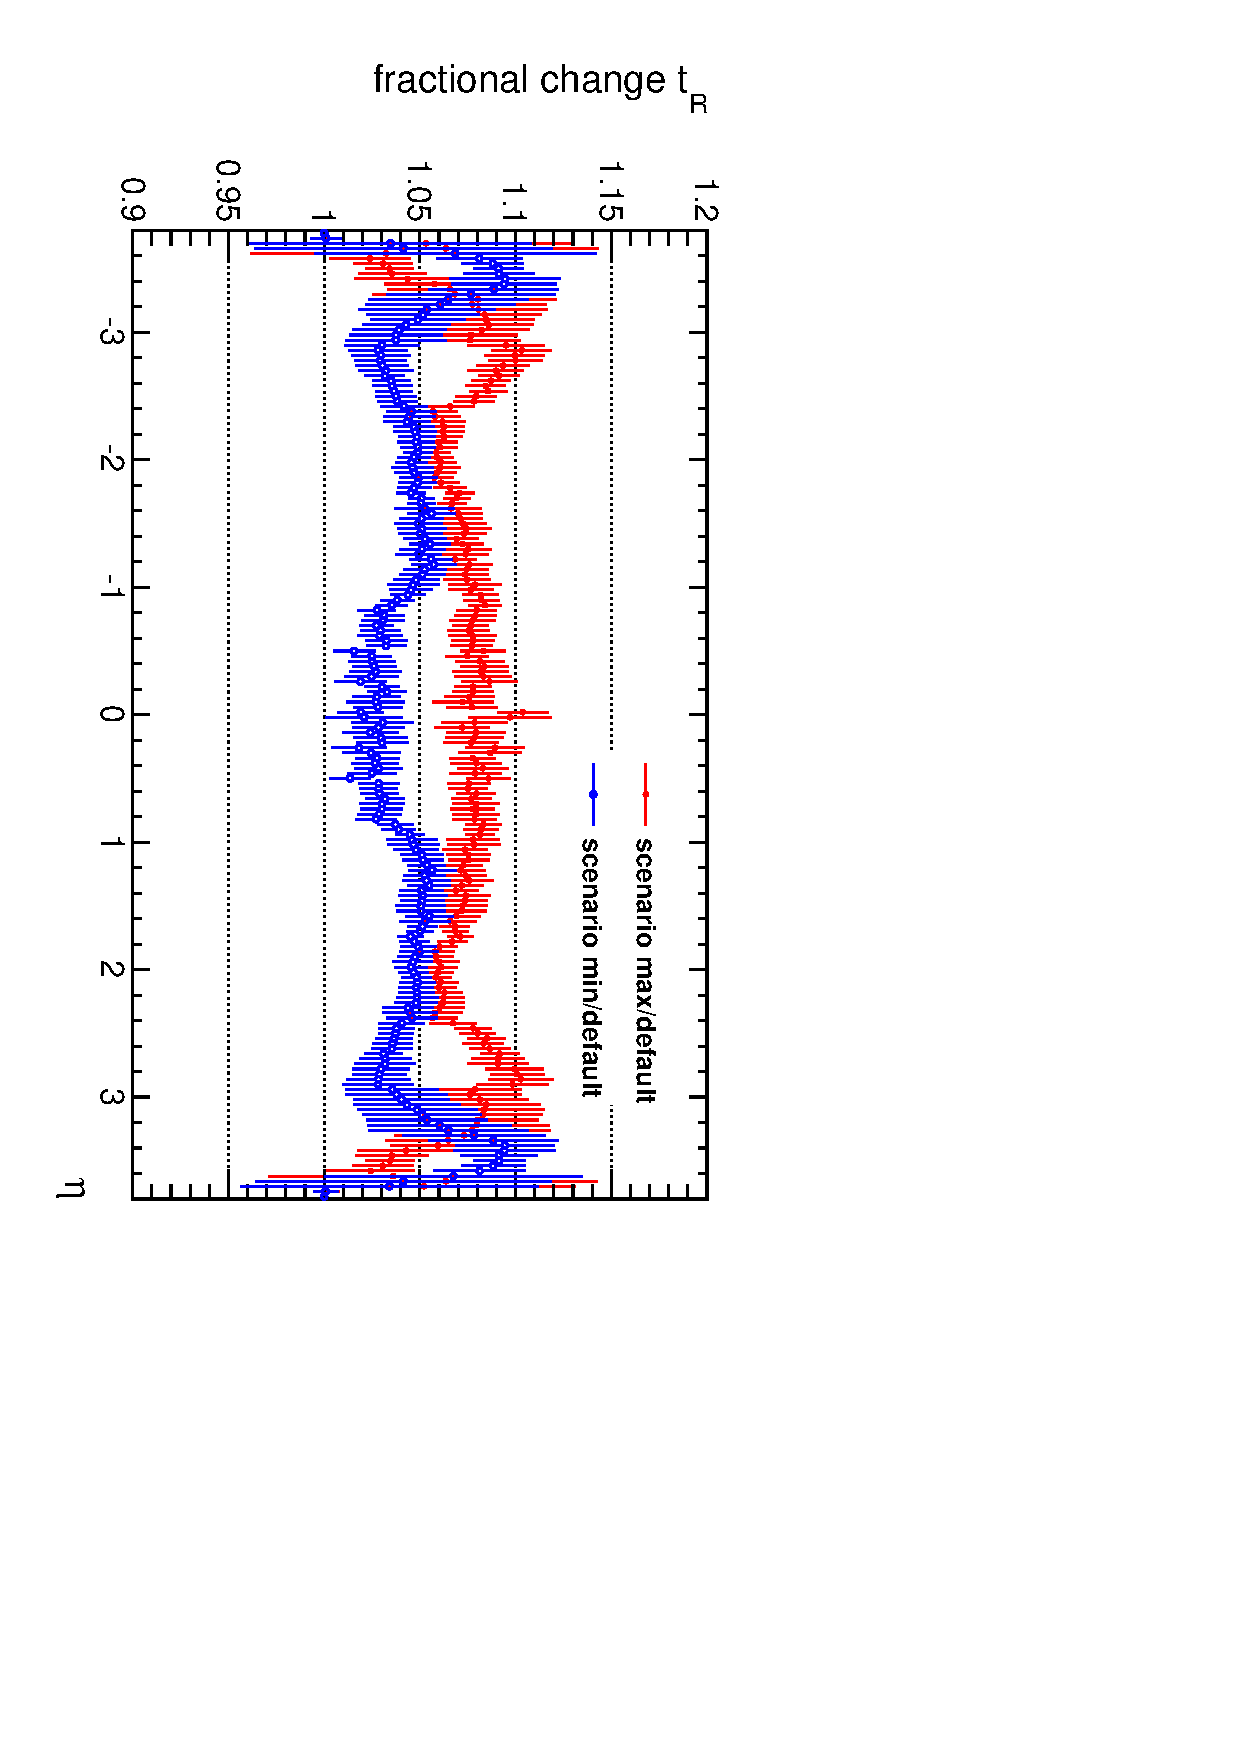
\includegraphics[width=0.5\textwidth,angle=90]{fig/lambda0minmax.pdf}
\end{center}
\caption{Fractional change of $\TI$ with respect the CMSSW setting
  for the $\kvect^{\rm I}_{max}$ and $\kvect^{\rm I}_{min}$ scenarios.
  An uniform increase of the Tracker mass of 5\% would correspond
  to a horizontal line at 1.05.}
\label{fig:lambda0minmax}
\end{figure}

\clearpage

\appendix
\numberwithin{table}{section}
\section{Tables of components mass.}
\label{compositionAppendix}

\vskip 1cm

\begin{table}[h]
\begin{center}
\begin{tabular}{clrrrrrr}
  &           & \multicolumn{2}{c}{Weight} & \multicolumn{2}{c}{Total} & \multicolumn{2}{c}{Remaining} \\ 
  & Name      & [kg]    & Fraction & [kg]  & Fraction & [kg]   & Fraction \\ 
 \hline 
 1 &          CarbonFiber &  13.618 & 17.770\% &  13.618 & 17.770\%  &  63.016 & 82.230\% \\
 2 &               Copper &  10.621 & 13.859\% &  24.239 & 31.630\%  &  52.395 & 68.370\% \\
 3 &                C6F14 &   8.716 & 11.374\% &  32.955 & 43.003\%  &  43.679 & 56.997\% \\
 4 &            Aluminium &   8.588 & 11.207\% &  41.543 & 54.210\%  &  35.091 & 45.790\% \\
 5 &                   PE &   7.944 & 10.366\% &  49.487 & 64.576\%  &  27.147 & 35.424\% \\
 6 &                  FR4 &   7.105 & 9.272\% &  56.593 & 73.847\%  &  20.042 & 26.153\% \\
 7 &                Epoxy &   6.124 & 7.991\% &  62.717 & 81.839\%  &  13.918 & 18.161\% \\
 8 &                Steel &   5.505 & 7.184\% &  68.222 & 89.023\%  &   8.413 & 10.977\% \\
 9 &             Acrylate &   4.558 & 5.948\% &  72.780 & 94.971\%  &   3.854 & 5.029\% \\
10 &              Silicon &   0.995 & 1.298\% &  73.775 & 96.269\%  &   2.860 & 3.731\% \\
11 &                Nomex &   0.720 & 0.939\% &  74.495 & 97.208\%  &   2.140 & 2.792\% \\
12 &               Kapton &   0.420 & 0.548\% &  74.914 & 97.755\%  &   1.720 & 2.245\% \\
13 &              Ceramic &   0.402 & 0.525\% &  75.317 & 98.280\%  &   1.318 & 1.720\% \\
14 &          SiliconeGel &   0.379 & 0.494\% &  75.695 & 98.774\%  &   0.939 & 1.226\% \\
15 &               Kevlar &   0.278 & 0.363\% &  75.973 & 99.137\%  &   0.661 & 0.863\% \\
16 &              Solders &   0.197 & 0.257\% &  76.170 & 99.394\%  &   0.464 & 0.606\% \\
17 &                Brass &   0.184 & 0.240\% &  76.354 & 99.634\%  &   0.280 & 0.366\% \\
18 &                  G10 &   0.134 & 0.175\% &  76.488 & 99.809\%  &   0.146 & 0.191\% \\
19 &                 BaTi &   0.117 & 0.152\% &  76.605 & 99.961\%  &   0.030 & 0.039\% \\
20 &                 Gold &   0.018 & 0.023\% &  76.623 & 99.984\%  &   0.012 & 0.016\% \\
21 &               Nickel &   0.009 & 0.011\% &  76.631 & 99.996\%  &   0.003 & 0.004\% \\
22 &                  Air &   0.003 & 0.004\% &  76.635 & 100.000\%  &   0.000 & 0.000\% \\
 \hline 
  & Total &   76.635 & 100.000\% & & & & \\ 

\end{tabular}
\caption{Mass of the basic components in the Pixel Barrel volume.}
\end{center}
\end{table}

\begin{table}[h]
\begin{center}
\begin{tabular}{clrrrrrr}
  &           & \multicolumn{2}{c}{Weight} & \multicolumn{2}{c}{Total} & \multicolumn{2}{c}{Remaining} \\ 
  & Name      & [kg]    & Fraction & [kg]  & Fraction & [kg]   & Fraction \\ 
 \hline 
 1 &          CarbonFiber &   3.633 & 25.995\% &   3.633 & 25.995\%  &  10.344 & 74.005\% \\
 2 &               Bronze &   2.656 & 19.001\% &   6.289 & 44.996\%  &   7.688 & 55.004\% \\
 3 &            Aluminium &   2.572 & 18.400\% &   8.861 & 63.395\%  &   5.116 & 36.605\% \\
 4 &                C6F14 &   1.532 & 10.958\% &  10.393 & 74.353\%  &   3.585 & 25.647\% \\
 5 &                   PE &   1.127 & 8.065\% &  11.520 & 82.418\%  &   2.457 & 17.582\% \\
 6 &                  G10 &   0.781 & 5.587\% &  12.301 & 88.005\%  &   1.677 & 11.995\% \\
 7 &               Copper &   0.430 & 3.074\% &  12.731 & 91.079\%  &   1.247 & 8.921\% \\
 8 &              Silicon &   0.393 & 2.811\% &  13.123 & 93.890\%  &   0.854 & 6.110\% \\
 9 &            Beryllium &   0.380 & 2.718\% &  13.503 & 96.608\%  &   0.474 & 3.392\% \\
10 &               Kapton &   0.231 & 1.652\% &  13.734 & 98.260\%  &   0.243 & 1.740\% \\
11 &              Ceramic &   0.076 & 0.540\% &  13.810 & 98.800\%  &   0.168 & 1.200\% \\
12 &          SiliconeGel &   0.063 & 0.453\% &  13.873 & 99.254\%  &   0.104 & 0.746\% \\
13 &                Epoxy &   0.044 & 0.318\% &  13.918 & 99.572\%  &   0.060 & 0.428\% \\
14 &                 BaTi &   0.028 & 0.202\% &  13.946 & 99.774\%  &   0.032 & 0.226\% \\
15 &              Solders &   0.027 & 0.193\% &  13.973 & 99.967\%  &   0.005 & 0.033\% \\
16 &        SiliconNoSens &   0.005 & 0.033\% &  13.977 & 100.000\%  &   0.000 & 0.000\% \\
 \hline 
  & Total &   13.977 & 100.000\% & & & & \\ 

\end{tabular}
\caption{Mass of the basic components in the Pixel Forward half located at $z>0$; the Pixel Forward half located at $z<0$ is identical.}
\end{center}
\end{table}

\begin{table}[h]
\begin{center}
\begin{tabular}{clrrrrrr}
  &           & \multicolumn{2}{c}{Weight} & \multicolumn{2}{c}{Total} & \multicolumn{2}{c}{Remaining} \\ 
  & Name      & [kg]    & Fraction & [kg]  & Fraction & [kg]   & Fraction \\ 
 \hline 
 1 &          CarbonFiber &  62.121 & 29.219\% &  62.121 & 29.219\%  & 150.485 & 70.781\% \\
 2 &            Aluminium &  32.724 & 15.392\% &  94.845 & 44.611\%  & 117.760 & 55.389\% \\
 3 &               Copper &  21.914 & 10.307\% & 116.759 & 54.918\%  &  95.846 & 45.082\% \\
 4 &              Silicon &  15.297 & 7.195\% & 132.056 & 62.113\%  &  80.550 & 37.887\% \\
 5 &                C6F14 &  15.210 & 7.154\% & 147.266 & 69.267\%  &  65.340 & 30.733\% \\
 6 &               Kapton &  14.339 & 6.745\% & 161.605 & 76.011\%  &  51.001 & 23.989\% \\
 7 &                   PE &  10.258 & 4.825\% & 171.863 & 80.837\%  &  40.743 & 19.163\% \\
 8 &              Ceramic &   8.885 & 4.179\% & 180.748 & 85.016\%  &  31.858 & 14.984\% \\
 9 &                  FR4 &   8.516 & 4.005\% & 189.264 & 89.021\%  &  23.342 & 10.979\% \\
10 &               Bronze &   5.199 & 2.445\% & 194.462 & 91.466\%  &  18.143 & 8.534\% \\
11 &                  G10 &   4.743 & 2.231\% & 199.205 & 93.697\%  &  13.400 & 6.303\% \\
12 &                Epoxy &   4.399 & 2.069\% & 203.604 & 95.766\%  &   9.002 & 4.234\% \\
13 &          SiliconeGel &   2.361 & 1.110\% & 205.965 & 96.876\%  &   6.641 & 3.124\% \\
14 &    BorosilicateGlass &   2.183 & 1.027\% & 208.148 & 97.903\%  &   4.458 & 2.097\% \\
15 &             Acrylate &   1.471 & 0.692\% & 209.618 & 98.595\%  &   2.987 & 1.405\% \\
16 &                 BaTi &   1.104 & 0.519\% & 210.722 & 99.114\%  &   1.883 & 0.886\% \\
17 &        SiliconNoSens &   1.050 & 0.494\% & 211.772 & 99.608\%  &   0.833 & 0.392\% \\
18 &                 Iron &   0.346 & 0.163\% & 212.119 & 99.771\%  &   0.487 & 0.229\% \\
19 &              Solders &   0.252 & 0.118\% & 212.370 & 99.889\%  &   0.235 & 0.111\% \\
20 &               Quartz &   0.101 & 0.047\% & 212.471 & 99.937\%  &   0.135 & 0.063\% \\
21 &                 Gold &   0.065 & 0.030\% & 212.536 & 99.967\%  &   0.070 & 0.033\% \\
22 &                Brass &   0.040 & 0.019\% & 212.576 & 99.986\%  &   0.030 & 0.014\% \\
23 &            Resistors &   0.030 & 0.014\% & 212.606 & 100.000\%  &   0.000 & 0.000\% \\
 \hline 
  & Total &  212.606 & 100.000\% & & & & \\ 

\end{tabular}
\caption{Mass of the basic components in the TIB volume.}
\end{center}
\end{table}

\begin{table}[h]
\begin{center}
\begin{tabular}{clrrrrrr}
  &           & \multicolumn{2}{c}{Weight} & \multicolumn{2}{c}{Total} & \multicolumn{2}{c}{Remaining} \\ 
  & Name      & [kg]    & Fraction & [kg]  & Fraction & [kg]   & Fraction \\ 
 \hline 
 1 &          CarbonFiber &  16.442 & 42.490\% &  16.442 & 42.490\%  &  22.255 & 57.510\% \\
 2 &            Aluminium &   4.079 & 10.540\% &  20.521 & 53.030\%  &  18.176 & 46.970\% \\
 3 &               Copper &   2.893 & 7.475\% &  23.414 & 60.506\%  &  15.283 & 39.494\% \\
 4 &               Kapton &   2.686 & 6.942\% &  26.100 & 67.448\%  &  12.597 & 32.552\% \\
 5 &              Silicon &   2.670 & 6.900\% &  28.771 & 74.348\%  &   9.927 & 25.652\% \\
 6 &              Ceramic &   1.847 & 4.772\% &  30.617 & 79.120\%  &   8.080 & 20.880\% \\
 7 &                Nomex &   1.623 & 4.195\% &  32.240 & 83.315\%  &   6.457 & 16.685\% \\
 8 &                C6F14 &   1.547 & 3.998\% &  33.788 & 87.313\%  &   4.910 & 12.687\% \\
 9 &                  FR4 &   1.211 & 3.129\% &  34.998 & 90.442\%  &   3.699 & 9.558\% \\
10 &                Epoxy &   1.018 & 2.630\% &  36.016 & 93.072\%  &   2.681 & 6.928\% \\
11 &                   PE &   0.772 & 1.996\% &  36.788 & 95.067\%  &   1.909 & 4.933\% \\
12 &    BorosilicateGlass &   0.643 & 1.661\% &  37.431 & 96.728\%  &   1.266 & 3.272\% \\
13 &               Bronze &   0.305 & 0.789\% &  37.737 & 97.518\%  &   0.961 & 2.482\% \\
14 &          SiliconeGel &   0.279 & 0.720\% &  38.015 & 98.237\%  &   0.682 & 1.763\% \\
15 &             Acrylate &   0.246 & 0.635\% &  38.261 & 98.872\%  &   0.436 & 1.128\% \\
16 &        SiliconNoSens &   0.159 & 0.412\% &  38.420 & 99.284\%  &   0.277 & 0.716\% \\
17 &                 BaTi &   0.152 & 0.393\% &  38.572 & 99.677\%  &   0.125 & 0.323\% \\
18 &                 Iron &   0.048 & 0.125\% &  38.621 & 99.802\%  &   0.077 & 0.198\% \\
19 &              Solders &   0.037 & 0.095\% &  38.657 & 99.897\%  &   0.040 & 0.103\% \\
20 &               Nickel &   0.018 & 0.046\% &  38.675 & 99.943\%  &   0.022 & 0.057\% \\
21 &               Quartz &   0.017 & 0.044\% &  38.692 & 99.987\%  &   0.005 & 0.013\% \\
22 &            Resistors &   0.005 & 0.013\% &  38.697 & 100.000\%  &   0.000 & 0.000\% \\
 \hline 
  & Total &   38.697 & 100.000\% & & & & \\ 

\end{tabular}
\caption{Mass of the basic components in the forward TID volume; backward TID volume is identical.}
\end{center}
\end{table}

\begin{table}[h]
\begin{center}
\begin{tabular}{clrrrrrr}
  &           & \multicolumn{2}{c}{Mass} & \multicolumn{2}{c}{Total} & \multicolumn{2}{c}{Remaining} \\ 
  & Name      & [kg]    & Fraction & [kg]  & Fraction & [kg]   & Fraction \\ 
 \hline 
 1 &               Copper &  56.040 & 26.020\% &  56.040 & 26.020\%  & 159.338 & 73.980\% \\
 2 &            Aluminium &  51.110 & 23.730\% & 107.150 & 49.750\%  & 108.228 & 50.250\% \\
 3 &                   PE &  42.186 & 19.587\% & 149.336 & 69.337\%  &  66.042 & 30.663\% \\
 4 &                C6F14 &  18.620 & 8.645\% & 167.956 & 77.982\%  &  47.422 & 22.018\% \\
 5 &                  FR4 &  14.332 & 6.654\% & 182.289 & 84.636\%  &  33.090 & 15.364\% \\
 6 &          CarbonFiber &   7.615 & 3.536\% & 189.904 & 88.172\%  &  25.474 & 11.828\% \\
 7 &             Acrylate &   4.949 & 2.298\% & 194.853 & 90.470\%  &  20.525 & 9.530\% \\
 8 &               Bronze &   4.393 & 2.040\% & 199.245 & 92.510\%  &  16.133 & 7.490\% \\
 9 &                Brass &   3.282 & 1.524\% & 202.527 & 94.033\%  &  12.851 & 5.967\% \\
10 &               Kapton &   3.017 & 1.401\% & 205.544 & 95.434\%  &   9.834 & 4.566\% \\
11 &               Silver &   2.468 & 1.146\% & 208.012 & 96.580\%  &   7.366 & 3.420\% \\
12 &              Solders &   1.495 & 0.694\% & 209.507 & 97.274\%  &   5.871 & 2.726\% \\
13 &                 Iron &   1.428 & 0.663\% & 210.935 & 97.937\%  &   4.443 & 2.063\% \\
14 &               Kevlar &   1.118 & 0.519\% & 212.053 & 98.456\%  &   3.325 & 1.544\% \\
15 &              Ceramic &   0.893 & 0.415\% & 212.946 & 98.871\%  &   2.432 & 1.129\% \\
16 &          SiliconeGel &   0.751 & 0.349\% & 213.698 & 99.220\%  &   1.680 & 0.780\% \\
17 &               Quartz &   0.694 & 0.322\% & 214.391 & 99.542\%  &   0.987 & 0.458\% \\
18 &                Steel &   0.471 & 0.218\% & 214.862 & 99.760\%  &   0.516 & 0.240\% \\
19 &                 Gold &   0.215 & 0.100\% & 215.077 & 99.860\%  &   0.302 & 0.140\% \\
20 &                Epoxy &   0.186 & 0.086\% & 215.262 & 99.946\%  &   0.116 & 0.054\% \\
21 &                  G10 &   0.085 & 0.040\% & 215.348 & 99.986\%  &   0.031 & 0.014\% \\
22 &                Nomex &   0.031 & 0.014\% & 215.378 & 100.000\%  &   0.000 & 0.000\% \\
 \hline 
  & Total &  215.378 & 100.000\% & & & & \\ 

\end{tabular}
\caption{Mass of the basic components in the forward TIB and TID service volume; the backward replica is identical.}
\end{center}
\end{table}

\begin{table}[h]
\begin{center}
\begin{tabular}{clrrrrrr}
  &           & \multicolumn{2}{c}{Mass} & \multicolumn{2}{c}{Total} & \multicolumn{2}{c}{Remaining} \\ 
  & Name      & [kg]    & Fraction & [kg]  & Fraction & [kg]   & Fraction \\ 
 \hline 
 1 &          CarbonFiber & 263.406 & 25.337\% & 263.406 & 25.337\%  & 776.184 & 74.663\% \\
 2 &               Copper & 124.997 & 12.024\% & 388.403 & 37.361\%  & 651.187 & 62.639\% \\
 3 &            Aluminium & 121.048 & 11.644\% & 509.451 & 49.005\%  & 530.139 & 50.995\% \\
 4 &              Silicon & 110.498 & 10.629\% & 619.949 & 59.634\%  & 419.641 & 40.366\% \\
 5 &                  G10 &  99.293 & 9.551\% & 719.242 & 69.185\%  & 320.347 & 30.815\% \\
 6 &                C6F14 &  86.370 & 8.308\% & 805.612 & 77.493\%  & 233.977 & 22.507\% \\
 7 &                   PE &  75.903 & 7.301\% & 881.515 & 84.795\%  & 158.074 & 15.205\% \\
 8 &              Ceramic &  36.157 & 3.478\% & 917.671 & 88.272\%  & 121.918 & 11.728\% \\
 9 &               Kapton &  21.757 & 2.093\% & 939.428 & 90.365\%  & 100.161 & 9.635\% \\
10 &                Epoxy &  20.287 & 1.951\% & 959.715 & 92.317\%  &  79.874 & 7.683\% \\
11 &                Nomex &  14.346 & 1.380\% & 974.061 & 93.697\%  &  65.528 & 6.303\% \\
12 &                 CuNi &  13.941 & 1.341\% & 988.002 & 95.038\%  &  51.587 & 4.962\% \\
13 &          SiliconeGel &  13.320 & 1.281\% & 1001.323 & 96.319\%  &  38.267 & 3.681\% \\
14 &    BorosilicateGlass &   8.799 & 0.846\% & 1010.122 & 97.165\%  &  29.468 & 2.835\% \\
15 &             Acrylate &   8.130 & 0.782\% & 1018.252 & 97.947\%  &  21.338 & 2.053\% \\
16 &                 BaTi &   7.811 & 0.751\% & 1026.063 & 98.699\%  &  13.527 & 1.301\% \\
17 &               Silver &   4.914 & 0.473\% & 1030.976 & 99.172\%  &   8.613 & 0.828\% \\
18 &               Kevlar &   2.603 & 0.250\% & 1033.580 & 99.422\%  &   6.010 & 0.578\% \\
19 &                Steel &   1.462 & 0.141\% & 1035.042 & 99.563\%  &   4.547 & 0.437\% \\
20 &               Quartz &   1.231 & 0.118\% & 1036.274 & 99.681\%  &   3.316 & 0.319\% \\
21 &        SiliconNoSens &   1.137 & 0.109\% & 1037.411 & 99.790\%  &   2.178 & 0.210\% \\
22 &              Solders &   1.100 & 0.106\% & 1038.511 & 99.896\%  &   1.078 & 0.104\% \\
23 &                Brass &   0.750 & 0.072\% & 1039.261 & 99.968\%  &   0.328 & 0.032\% \\
24 &                 Iron &   0.273 & 0.026\% & 1039.534 & 99.995\%  &   0.055 & 0.005\% \\
25 &            Resistors &   0.055 & 0.005\% & 1039.589 & 100.000\%  &   0.000 & 0.000\% \\
 \hline 
  & Total & 1039.589 & 100.000\% & & & & \\ 

\end{tabular}
\caption{Mass of the basic components in the TOB volume.}
\end{center}
\end{table}

\begin{table}[h]
\begin{center}
\begin{tabular}{clrrrrrr}
  &           & \multicolumn{2}{c}{Mass} & \multicolumn{2}{c}{Total} & \multicolumn{2}{c}{Remaining} \\ 
  & Name      & [kg]    & Fraction & [kg]  & Fraction & [kg]   & Fraction \\ 
 \hline 
 1 &          CarbonFiber & 194.292 & 29.105\% & 194.292 & 29.105\%  & 473.272 & 70.895\% \\
 2 &                   PE &  64.880 & 9.719\% & 259.171 & 38.823\%  & 408.392 & 61.177\% \\
 3 &            Aluminium &  63.340 & 9.488\% & 322.511 & 48.312\%  & 345.052 & 51.688\% \\
 4 &               Copper &  49.541 & 7.421\% & 372.053 & 55.733\%  & 295.511 & 44.267\% \\
 5 &              Silicon &  46.466 & 6.960\% & 418.518 & 62.693\%  & 249.045 & 37.307\% \\
 6 &                Nomex &  35.256 & 5.281\% & 453.774 & 67.975\%  & 213.789 & 32.025\% \\
 7 &                C6F14 &  32.197 & 4.823\% & 485.971 & 72.798\%  & 181.592 & 27.202\% \\
 8 &                Steel &  30.539 & 4.575\% & 516.510 & 77.373\%  & 151.053 & 22.627\% \\
 9 &                  FR4 &  28.236 & 4.230\% & 544.746 & 81.602\%  & 122.817 & 18.398\% \\
10 &             Graphite &  25.118 & 3.763\% & 569.865 & 85.365\%  &  97.698 & 14.635\% \\
11 &              Ceramic &  19.994 & 2.995\% & 589.859 & 88.360\%  &  77.704 & 11.640\% \\
12 &               Quartz &  17.876 & 2.678\% & 607.735 & 91.038\%  &  59.829 & 8.962\% \\
13 &             Titanium &  15.733 & 2.357\% & 623.468 & 93.395\%  &  44.095 & 6.605\% \\
14 &                Epoxy &  11.426 & 1.712\% & 634.894 & 95.106\%  &  32.670 & 4.894\% \\
15 &               Kapton &  10.469 & 1.568\% & 645.362 & 96.674\%  &  22.201 & 3.326\% \\
16 &    BorosilicateGlass &   5.433 & 0.814\% & 650.796 & 97.488\%  &  16.767 & 2.512\% \\
17 &                Brass &   3.696 & 0.554\% & 654.492 & 98.042\%  &  13.072 & 1.958\% \\
18 &               Silver &   2.659 & 0.398\% & 657.151 & 98.440\%  &  10.412 & 1.560\% \\
19 &              Solders &   2.600 & 0.389\% & 659.751 & 98.830\%  &   7.812 & 1.170\% \\
20 &             Acrylate &   2.526 & 0.378\% & 662.277 & 99.208\%  &   5.287 & 0.792\% \\
21 &                  G10 &   2.139 & 0.320\% & 664.415 & 99.528\%  &   3.148 & 0.472\% \\
22 &                 Peek &   1.786 & 0.268\% & 666.201 & 99.796\%  &   1.362 & 0.204\% \\
23 &        SiliconNoSens &   0.805 & 0.121\% & 667.006 & 99.917\%  &   0.557 & 0.083\% \\
24 &                 BaTi &   0.222 & 0.033\% & 667.229 & 99.950\%  &   0.334 & 0.050\% \\
25 &                 Iron &   0.173 & 0.026\% & 667.402 & 99.976\%  &   0.162 & 0.024\% \\
26 &               Nickel &   0.109 & 0.016\% & 667.511 & 99.992\%  &   0.053 & 0.008\% \\
27 &            Resistors &   0.039 & 0.006\% & 667.549 & 99.998\%  &   0.014 & 0.002\% \\
28 &                  Air &   0.008 & 0.001\% & 667.557 & 99.999\%  &   0.006 & 0.001\% \\
29 &                 Gold &   0.006 & 0.001\% & 667.563 & 100.000\%  &   0.000 & 0.000\% \\
 \hline 
  & Total &  667.563 & 100.000\% & & & & \\ 

\end{tabular}
\caption{Mass of the basic components in one of the two TEC volume replicas.}
\end{center}
\end{table}

\begin{table}[h]
\begin{center}
\begin{tabular}{clrrrrrr}
  &           & \multicolumn{2}{c}{Mass} & \multicolumn{2}{c}{Total} & \multicolumn{2}{c}{Remaining} \\ 
  & Name      & [kg]    & Fraction & [kg]  & Fraction & [kg]   & Fraction \\ 
 \hline 
 1 &               Copper & 110.151 & 54.453\% & 110.151 & 54.453\%  &  92.134 & 45.547\% \\
 2 &          CarbonFiber &  34.079 & 16.847\% & 144.229 & 71.300\%  &  58.056 & 28.700\% \\
 3 &            Aluminium &  22.036 & 10.893\% & 166.265 & 82.193\%  &  36.020 & 17.807\% \\
 4 &                   PE &  21.289 & 10.524\% & 187.554 & 92.718\%  &  14.731 & 7.282\% \\
 5 &                C6F14 &   5.995 & 2.963\% & 193.548 & 95.681\%  &   8.737 & 4.319\% \\
 6 &               Kapton &   4.262 & 2.107\% & 197.810 & 97.788\%  &   4.475 & 2.212\% \\
 7 &                Steel &   2.152 & 1.064\% & 199.962 & 98.852\%  &   2.323 & 1.148\% \\
 8 &               Nickel &   0.707 & 0.349\% & 200.668 & 99.201\%  &   1.616 & 0.799\% \\
 9 &                Epoxy &   0.448 & 0.221\% & 201.116 & 99.422\%  &   1.169 & 0.578\% \\
10 &               Silver &   0.441 & 0.218\% & 201.557 & 99.640\%  &   0.727 & 0.360\% \\
11 &                Nomex &   0.306 & 0.151\% & 201.863 & 99.791\%  &   0.422 & 0.209\% \\
12 &               Quartz &   0.260 & 0.128\% & 202.123 & 99.920\%  &   0.162 & 0.080\% \\
13 &             Titanium &   0.120 & 0.059\% & 202.243 & 99.979\%  &   0.042 & 0.021\% \\
14 &                  FR4 &   0.024 & 0.012\% & 202.267 & 99.991\%  &   0.018 & 0.009\% \\
15 &        SiliconNoSens &   0.018 & 0.009\% & 202.285 & 100.000\%  &   0.000 & 0.000\% \\
 \hline 
  & Total &  202.285 & 100.000\% & & & & \\ 

\end{tabular}
\caption{Mass of the basic components in one of the two Tracker Bulkhead volume replicas.}
\end{center}
\end{table}

\begin{table}[h]
\begin{center}
\begin{tabular}{clrrrrrr}
  &           & \multicolumn{2}{c}{Mass} & \multicolumn{2}{c}{Total} & \multicolumn{2}{c}{Remaining} \\ 
  & Name      & [kg]    & Fraction & [kg]  & Fraction & [kg]   & Fraction \\ 
 \hline 
 1 &          CarbonFiber & 293.221 & 54.572\% & 293.221 & 54.572\%  & 244.094 & 45.428\% \\
 2 &            Aluminium & 146.301 & 27.228\% & 439.522 & 81.800\%  &  97.792 & 18.200\% \\
 3 &                Nomex &  33.834 & 6.297\% & 473.356 & 88.097\%  &  63.959 & 11.903\% \\
 4 &                C6F14 &  28.854 & 5.370\% & 502.209 & 93.467\%  &  35.105 & 6.533\% \\
 5 &             Rohacell &  14.539 & 2.706\% & 516.749 & 96.172\%  &  20.566 & 3.828\% \\
 6 &                Steel &   8.230 & 1.532\% & 524.979 & 97.704\%  &  12.335 & 2.296\% \\
 7 &           Inconel600 &   7.426 & 1.382\% & 532.405 & 99.086\%  &   4.910 & 0.914\% \\
 8 &               Kapton &   4.910 & 0.914\% & 537.314 & 100.000\%  &   0.000 & 0.000\% \\
 \hline 
  & Total &  537.314 & 100.000\% & & & & \\ 

\end{tabular}
\caption{Mass of the basic components of the Tracker Outer Cylinder volume.}
\end{center}
\end{table}

\clearpage

\section{Tables of material category mass per subdetector}
\label{categoriesAppendix}

\vskip 1cm


\begin{table}[h]
\begin{center}
\begin{tabular}{clrrrrrr}
  &           & \multicolumn{2}{c}{Mass} & \multicolumn{2}{c}{Total} & \multicolumn{2}{c}{Remaining} \\ 
  & Name      & [kg]    & Fraction & [kg]  & Fraction & [kg]   & Fraction \\ 
 \hline 
 1 &          CarbonFiber &  13.618 & 17.770\% &  13.618 & 17.770\%  &  63.016 & 82.230\% \\
 2 &     OrganicMaterials &  13.200 & 17.225\% &  26.818 & 34.995\%  &  49.816 & 65.005\% \\
 3 &    CopperAndCuAlloys &  10.805 & 14.099\% &  37.623 & 49.094\%  &  39.011 & 50.906\% \\
 4 &                C6F14 &   8.716 & 11.374\% &  46.339 & 60.468\%  &  30.295 & 39.532\% \\
 5 &            Aluminium &   8.588 & 11.207\% &  54.928 & 71.675\%  &  21.707 & 28.325\% \\
 6 &  FiberGlassLaminated &   7.239 & 9.447\% &  62.167 & 81.121\%  &  14.468 & 18.879\% \\
 7 &        GlueAndResins &   6.503 & 8.485\% &  68.670 & 89.607\%  &   7.965 & 10.393\% \\
 8 &          OtherMetals &   5.523 & 7.207\% &  74.192 & 96.813\%  &   2.442 & 3.187\% \\
 9 &              SiliconSensitive &   0.995 & 1.298\% &  75.187 & 98.111\%  &   1.447 & 1.889\% \\
10 &      OtherMechStruct &   0.720 & 0.939\% &  75.907 & 99.050\%  &   0.728 & 0.950\% \\
11 &      InorganicOxides &   0.402 & 0.525\% &  76.309 & 99.575\%  &   0.325 & 0.425\% \\
12 & ElectronicComponents &   0.322 & 0.421\% &  76.631 & 99.996\%  &   0.003 & 0.004\% \\
13 &                  Air &   0.003 & 0.004\% &  76.635 & 100.000\%  &   0.000 & 0.000\% \\
 \hline 
  & Total &   76.635 & 100.000\% & & & & \\ 

\end{tabular}
\caption{Mass per material category in the Pixel Barrel volume.}
\end{center}
\end{table}

\begin{table}[h]
\begin{center}
\begin{tabular}{clrrrrrr}
  &           & \multicolumn{2}{c}{Mass} & \multicolumn{2}{c}{Total} & \multicolumn{2}{c}{Remaining} \\ 
  & Name      & [kg]    & Fraction & [kg]  & Fraction & [kg]   & Fraction \\ 
 \hline 
 1 &          CarbonFiber &   3.633 & 25.995\% &   3.633 & 25.995\%  &  10.344 & 74.005\% \\
 2 &    CopperAndCuAlloys &   3.085 & 22.075\% &   6.719 & 48.069\%  &   7.259 & 51.931\% \\
 3 &            Aluminium &   2.572 & 18.400\% &   9.291 & 66.469\%  &   4.687 & 33.531\% \\
 4 &                C6F14 &   1.532 & 10.958\% &  10.822 & 77.427\%  &   3.155 & 22.573\% \\
 5 &     OrganicMaterials &   1.358 & 9.717\% &  12.181 & 87.144\%  &   1.797 & 12.856\% \\
 6 &  FiberGlassLaminated &   0.781 & 5.587\% &  12.961 & 92.731\%  &   1.016 & 7.269\% \\
 7 &              SiliconSensitive &   0.393 & 2.811\% &  13.354 & 95.542\%  &   0.623 & 4.458\% \\
 8 &          OtherMetals &   0.380 & 2.718\% &  13.734 & 98.260\%  &   0.243 & 1.740\% \\
 9 &        GlueAndResins &   0.108 & 0.772\% &  13.842 & 99.031\%  &   0.135 & 0.969\% \\
10 &      InorganicOxides &   0.076 & 0.540\% &  13.918 & 99.572\%  &   0.060 & 0.428\% \\
11 & ElectronicComponents &   0.060 & 0.428\% &  13.977 & 100.000\%  &   0.000 & 0.000\% \\
 \hline 
  & Total &   13.977 & 100.000\% & & & & \\ 

\end{tabular}
\caption{Mass per material category in the Pixel Forward half located at $z>0$; the Pixel Forward half located at $z<0$ is identical.}
\end{center}
\end{table}

\begin{table}[h]
\begin{center}
\begin{tabular}{clrrrrrr}
  &           & \multicolumn{2}{c}{Mass} & \multicolumn{2}{c}{Total} & \multicolumn{2}{c}{Remaining} \\ 
  & Name      & [kg]    & Fraction & [kg]  & Fraction & [kg]   & Fraction \\ 
 \hline 
 1 &          CarbonFiber &  62.121 & 29.219\% &  62.121 & 29.219\%  & 150.485 & 70.781\% \\
 2 &            Aluminium &  32.724 & 15.392\% &  94.845 & 44.611\%  & 117.760 & 55.389\% \\
 3 &    CopperAndCuAlloys &  27.153 & 12.772\% & 121.998 & 57.382\%  &  90.607 & 42.618\% \\
 4 &     OrganicMaterials &  26.068 & 12.261\% & 148.067 & 69.644\%  &  64.539 & 30.356\% \\
 5 &              SiliconSensitive &  15.297 & 7.195\% & 163.363 & 76.839\%  &  49.243 & 23.161\% \\
 6 &                C6F14 &  15.210 & 7.154\% & 178.573 & 83.992\%  &  34.033 & 16.008\% \\
 7 &  FiberGlassLaminated &  13.259 & 6.236\% & 191.831 & 90.229\%  &  20.774 & 9.771\% \\
 8 &      InorganicOxides &  11.169 & 5.253\% & 203.000 & 95.482\%  &   9.605 & 4.518\% \\
 9 &        GlueAndResins &   6.759 & 3.179\% & 209.759 & 98.661\%  &   2.846 & 1.339\% \\
10 & ElectronicComponents &   2.435 & 1.145\% & 212.195 & 99.807\%  &   0.411 & 0.193\% \\
11 &          OtherMetals &   0.411 & 0.193\% & 212.606 & 100.000\%  &   0.000 & 0.000\% \\
 \hline 
  & Total &  212.606 & 100.000\% & & & & \\ 

\end{tabular}
\caption{Mass per material category in the TIB volume.}
\end{center}
\end{table}

\begin{table}[h]
\begin{center}
\begin{tabular}{clrrrrrr}
  &           & \multicolumn{2}{c}{Weight} & \multicolumn{2}{c}{Total} & \multicolumn{2}{c}{Remaining} \\ 
  & Name      & [kg]    & Fraction & [kg]  & Fraction & [kg]   & Fraction \\ 
 \hline 
 1 &          CarbonFiber &  16.442 & 42.490\% &  16.442 & 42.490\%  &  22.255 & 57.510\% \\
 2 &            Aluminium &   4.079 & 10.540\% &  20.521 & 53.030\%  &  18.176 & 46.970\% \\
 3 &     OrganicMaterials &   3.704 & 9.573\% &  24.226 & 62.603\%  &  14.472 & 37.397\% \\
 4 &    CopperAndCuAlloys &   3.198 & 8.265\% &  27.424 & 70.868\%  &  11.273 & 29.132\% \\
 5 &              Silicon &   2.670 & 6.900\% &  30.094 & 77.768\%  &   8.603 & 22.232\% \\
 6 &      InorganicOxides &   2.506 & 6.476\% &  32.600 & 84.244\%  &   6.097 & 15.756\% \\
 7 &      OtherMechStruct &   1.623 & 4.195\% &  34.223 & 88.438\%  &   4.474 & 11.562\% \\
 8 &                C6F14 &   1.547 & 3.998\% &  35.770 & 92.437\%  &   2.927 & 7.563\% \\
 9 &        GlueAndResins &   1.296 & 3.350\% &  37.067 & 95.787\%  &   1.630 & 4.213\% \\
10 &  FiberGlassLaminated &   1.211 & 3.129\% &  38.277 & 98.916\%  &   0.420 & 1.084\% \\
11 & ElectronicComponents &   0.371 & 0.960\% &  38.649 & 99.875\%  &   0.048 & 0.125\% \\
12 &          OtherMetals &   0.048 & 0.125\% &  38.697 & 100.000\%  &   0.000 & 0.000\% \\
 \hline 
  & Total &   38.697 & 100.000\% & & & & \\ 

\end{tabular}
\caption{Mass per material category in the forward TID volume; backward TID volume is identical.}
\end{center}
\end{table}

\begin{table}[h]
\begin{center}
\begin{tabular}{clrrrrrr}
  &           & \multicolumn{2}{c}{Mass} & \multicolumn{2}{c}{Total} & \multicolumn{2}{c}{Remaining} \\ 
  & Name      & [kg]    & Fraction & [kg]  & Fraction & [kg]   & Fraction \\ 
 \hline 
 1 &    CopperAndCuAlloys &  63.715 & 29.583\% &  63.715 & 29.583\%  & 151.663 & 70.417\% \\
 2 &     OrganicMaterials &  51.270 & 23.805\% & 114.985 & 53.387\%  & 100.393 & 46.613\% \\
 3 &            Aluminium &  51.110 & 23.730\% & 166.095 & 77.118\%  &  49.283 & 22.882\% \\
 4 &                C6F14 &  18.620 & 8.645\% & 184.715 & 85.763\%  &  30.663 & 14.237\% \\
 5 &  FiberGlassLaminated &  14.417 & 6.694\% & 199.132 & 92.457\%  &  16.246 & 7.543\% \\
 6 &          CarbonFiber &   7.615 & 3.536\% & 206.748 & 95.993\%  &   8.630 & 4.007\% \\
 7 &          OtherMetals &   4.581 & 2.127\% & 211.329 & 98.120\%  &   4.049 & 1.880\% \\
 8 &      InorganicOxides &   1.587 & 0.737\% & 212.915 & 98.857\%  &   2.463 & 1.143\% \\
 9 & ElectronicComponents &   1.495 & 0.694\% & 214.410 & 99.551\%  &   0.968 & 0.449\% \\
10 &        GlueAndResins &   0.937 & 0.435\% & 215.348 & 99.986\%  &   0.031 & 0.014\% \\
11 &      OtherMechStruct &   0.031 & 0.014\% & 215.378 & 100.000\%  &   0.000 & 0.000\% \\
 \hline 
  & Total &  215.378 & 100.000\% & & & & \\ 

\end{tabular}
\caption{Mass per material category in the forward TIB and TID service volume; the backward replica is identical.}
\end{center}
\end{table}

\begin{table}[h]
\begin{center}
\begin{tabular}{clrrrrrr}
  &           & \multicolumn{2}{c}{Weight} & \multicolumn{2}{c}{Total} & \multicolumn{2}{c}{Remaining} \\ 
  & Name      & [kg]    & Fraction & [kg]  & Fraction & [kg]   & Fraction \\ 
 \hline 
 1 &          CarbonFiber & 263.406 & 25.337\% & 263.406 & 25.337\%  & 776.184 & 74.663\% \\
 2 &    CopperAndCuAlloys & 139.688 & 13.437\% & 403.094 & 38.774\%  & 636.496 & 61.226\% \\
 3 &            Aluminium & 121.048 & 11.644\% & 524.142 & 50.418\%  & 515.448 & 49.582\% \\
 4 &              Silicon & 110.498 & 10.629\% & 634.640 & 61.047\%  & 404.950 & 38.953\% \\
 5 &     OrganicMaterials & 108.393 & 10.427\% & 743.033 & 71.474\%  & 296.557 & 28.526\% \\
 6 &  FiberGlassLaminated &  99.293 & 9.551\% & 842.326 & 81.025\%  & 197.263 & 18.975\% \\
 7 &                C6F14 &  86.370 & 8.308\% & 928.696 & 89.333\%  & 110.893 & 10.667\% \\
 8 &      InorganicOxides &  46.187 & 4.443\% & 974.883 & 93.776\%  &  64.706 & 6.224\% \\
 9 &        GlueAndResins &  33.607 & 3.233\% & 1008.490 & 97.009\%  &  31.099 & 2.991\% \\
10 &      OtherMechStruct &  14.346 & 1.380\% & 1022.837 & 98.389\%  &  16.753 & 1.611\% \\
11 & ElectronicComponents &  10.103 & 0.972\% & 1032.940 & 99.360\%  &   6.650 & 0.640\% \\
12 &          OtherMetals &   6.650 & 0.640\% & 1039.589 & 100.000\%  &   0.000 & 0.000\% \\
 \hline 
  & Total & 1039.589 & 100.000\% & & & & \\ 

\end{tabular}
\caption{Mass per material category in the TOB volume.}
\end{center}
\end{table}

\begin{table}[h]
\begin{center}
\begin{tabular}{clrrrrrr}
  &           & \multicolumn{2}{c}{Mass} & \multicolumn{2}{c}{Total} & \multicolumn{2}{c}{Remaining} \\ 
  & Name      & [kg]    & Fraction & [kg]  & Fraction & [kg]   & Fraction \\ 
 \hline 
 1 &          CarbonFiber & 194.292 & 29.105\% & 194.292 & 29.105\%  & 473.272 & 70.895\% \\
 2 &     OrganicMaterials &  77.874 & 11.665\% & 272.166 & 40.770\%  & 395.398 & 59.230\% \\
 3 &            Aluminium &  63.340 & 9.488\% & 335.506 & 50.258\%  & 332.057 & 49.742\% \\
 4 &      OtherMechStruct &  62.160 & 9.312\% & 397.666 & 59.570\%  & 269.897 & 40.430\% \\
 5 &    CopperAndCuAlloys &  53.237 & 7.975\% & 450.904 & 67.545\%  & 216.660 & 32.455\% \\
 6 &          OtherMetals &  49.111 & 7.357\% & 500.015 & 74.901\%  & 167.548 & 25.099\% \\
 7 &              SiliconSensitive &  46.466 & 6.960\% & 546.480 & 81.862\%  & 121.083 & 18.138\% \\
 8 &      InorganicOxides &  43.303 & 6.487\% & 589.784 & 88.349\%  &  77.780 & 11.651\% \\
 9 &                C6F14 &  32.197 & 4.823\% & 621.980 & 93.172\%  &  45.583 & 6.828\% \\
10 &  FiberGlassLaminated &  30.375 & 4.550\% & 652.355 & 97.722\%  &  15.208 & 2.278\% \\
11 &        GlueAndResins &  11.426 & 1.712\% & 663.781 & 99.433\%  &   3.782 & 0.567\% \\
12 & ElectronicComponents &   3.775 & 0.565\% & 667.555 & 99.999\%  &   0.008 & 0.001\% \\
13 &                  Air &   0.008 & 0.001\% & 667.563 & 100.000\%  &   0.000 & 0.000\% \\
 \hline 
  & Total &  667.563 & 100.000\% & & & & \\ 

\end{tabular}
\caption{Mass per material category in one of the two TEC volume replicas.}
\end{center}
\end{table}

\begin{table}[h]
\begin{center}
\begin{tabular}{clrrrrrr}
  &           & \multicolumn{2}{c}{Mass} & \multicolumn{2}{c}{Total} & \multicolumn{2}{c}{Remaining} \\ 
  & Name      & [kg]    & Fraction & [kg]  & Fraction & [kg]   & Fraction \\ 
 \hline 
 1 &    CopperAndCuAlloys & 110.151 & 54.453\% & 110.151 & 54.453\%  &  92.134 & 45.547\% \\
 2 &          CarbonFiber &  34.079 & 16.847\% & 144.229 & 71.300\%  &  58.056 & 28.700\% \\
 3 &     OrganicMaterials &  25.551 & 12.631\% & 169.780 & 83.931\%  &  32.505 & 16.069\% \\
 4 &            Aluminium &  22.036 & 10.893\% & 191.816 & 94.825\%  &  10.469 & 5.175\% \\
 5 &                C6F14 &   5.995 & 2.963\% & 197.810 & 97.788\%  &   4.475 & 2.212\% \\
 6 &          OtherMetals &   2.713 & 1.341\% & 200.523 & 99.129\%  &   1.762 & 0.871\% \\
 7 & ElectronicComponents &   0.725 & 0.358\% & 201.248 & 99.487\%  &   1.037 & 0.513\% \\
 8 &        GlueAndResins &   0.448 & 0.221\% & 201.695 & 99.709\%  &   0.589 & 0.291\% \\
 9 &      OtherMechStruct &   0.306 & 0.151\% & 202.001 & 99.860\%  &   0.284 & 0.140\% \\
10 &      InorganicOxides &   0.260 & 0.128\% & 202.261 & 99.988\%  &   0.024 & 0.012\% \\
11 &  FiberGlassLaminated &   0.024 & 0.012\% & 202.285 & 100.000\%  &   0.000 & 0.000\% \\
 \hline 
  & Total &  202.285 & 100.000\% & & & & \\ 

\end{tabular}
\caption{Mass per material category in one of the two Tracker Bulkhead volume replicas.}
\end{center}
\end{table}

\begin{table}[h]
\begin{center}
\begin{tabular}{clrrrrrr}
  &           & \multicolumn{2}{c}{Weight} & \multicolumn{2}{c}{Total} & \multicolumn{2}{c}{Remaining} \\ 
  & Name      & [kg]    & Fraction & [kg]  & Fraction & [kg]   & Fraction \\ 
 \hline 
 1 &          CarbonFiber & 293.221 & 54.572\% & 293.221 & 54.572\%  & 244.094 & 45.428\% \\
 2 &            Aluminium & 146.301 & 27.228\% & 439.522 & 81.800\%  &  97.792 & 18.200\% \\
 3 &      OtherMechStruct &  48.373 & 9.003\% & 487.895 & 90.803\%  &  49.419 & 9.197\% \\
 4 &                C6F14 &  28.854 & 5.370\% & 516.749 & 96.172\%  &  20.566 & 3.828\% \\
 5 &          OtherMetals &  15.656 & 2.914\% & 532.405 & 99.086\%  &   4.910 & 0.914\% \\
 6 &     OrganicMaterials &   4.910 & 0.914\% & 537.314 & 100.000\%  &   0.000 & 0.000\% \\
 \hline 
  & Total &  537.314 & 100.000\% & & & & \\ 

\end{tabular}
\caption{Mass per material category of the Tracker Outer Cylinder volume.}
\end{center}
\end{table}

\end{document}

% LocalWords:  TODO
